% Informe final del proyecto de Machine Learning (Entregables 1 a 3: fuga de clientes, COFINFAD).
% Une la introducción, la sección de metodología (../Metodologia Entregable 3), la sección de resultados
% (../Resultados Entregable 3) y las conclusiones. Armar: python armar.py; compilar: python compilar.py (Tectonic).
\documentclass[11pt,a4paper]{article}

\usepackage[T1]{fontenc}
\usepackage[utf8]{inputenc}
\usepackage{lmodern}
\usepackage[spanish,es-tabla,es-noshorthands]{babel}
\usepackage[a4paper,textwidth=6.3in,textheight=9.4in,headheight=14pt]{geometry}
\usepackage{amsmath,amssymb,bm}
\usepackage{graphicx}
\usepackage{booktabs}
\usepackage{array}
\usepackage{caption}
\usepackage{algorithm}
\usepackage{algpseudocode}
\usepackage[authoryear,round]{natbib}
\usepackage[section]{placeins}
\usepackage{microtype}
\usepackage{xcolor}
\usepackage[colorlinks=true,linkcolor=blue!55!black,citecolor=blue!55!black,urlcolor=blue!55!black]{hyperref}

\graphicspath{{figures/}}
\captionsetup{font=small,labelfont=bf,width=0.95\linewidth}
% Las figuras grandes pueden ocupar casi toda una página sin irse al final de la sección.
\renewcommand{\topfraction}{0.95}
\renewcommand{\bottomfraction}{0.6}
\renewcommand{\textfraction}{0.05}
\renewcommand{\floatpagefraction}{0.7}
\widowpenalty=10000 \clubpenalty=10000
\setlength{\parskip}{3pt plus 1pt}
\setlength{\bibsep}{3pt plus 1pt}
\setcounter{tocdepth}{2}
\renewcommand{\algorithmicrequire}{\textbf{Entrada:}}
\renewcommand{\algorithmicensure}{\textbf{Salida:}}
\algrenewcommand\algorithmicfor{\textbf{para}}
\algrenewcommand\algorithmicdo{\textbf{hacer}}
\algrenewcommand\algorithmicend{\textbf{fin}}
\algrenewcommand\algorithmicif{\textbf{si}}
\algrenewcommand\algorithmicthen{\textbf{entonces}}
\algrenewcommand\algorithmicwhile{\textbf{mientras}}
\algrenewcommand\algorithmicreturn{\textbf{devolver}}
\floatname{algorithm}{Algoritmo}

% Notación (la de las dos secciones)
\newcommand{\R}{\mathbb{R}}
\newcommand{\E}{\mathbb{E}}
\newcommand{\X}{\mathcal{X}}
\newcommand{\yhat}{\hat{y}}
\newcommand{\cp}{\texttt{churn\_probability}}
\newcommand{\ap}{\texttt{active\_products}}
\newcommand{\auc}{\mathrm{AUC}}
\newcommand{\rmse}{\mathrm{RMSE}}

\title{\textbf{Predicción de la fuga de clientes de una \emph{fintech} con una Explainable Boosting Machine}\\[6pt]
\large Informe final del proyecto de Machine Learning (Entregables 1 a 3)}
\author{Valerie Martínez Pulido, Abrahan Basto Martínez y Rubén Esguerra Fernández\\[4pt]
\small Pregrado en Ciencia de Datos, Departamento de Matemáticas, Física y Ciencia de Datos\\
\small Universidad del Norte, Barranquilla, Colombia}
\date{Noviembre de 2026}

\begin{document}
\maketitle

\begin{abstract}
\noindent La fuga de clientes es uno de los problemas de predicción más frecuentes en los servicios financieros
digitales. Sobre el conjunto público COFINFAD (48.723 clientes de una \emph{fintech} colombiana) este proyecto
abordó, en tres entregas, la clasificación del cuarto de clientes de mayor riesgo y la regresión del puntaje de
propensión al abandono. Tras la auditoría de los datos y los modelos lineales de referencia de las dos primeras
entregas, se propone una \emph{Explainable Boosting Machine} (EBM), un modelo aditivo generalizado cuyas
funciones de forma se aprenden por \emph{boosting} cíclico de árboles pequeños, adaptada con pesos de clase y
una búsqueda multi-fidelidad, y se compara con los modelos del curso dentro de un pipeline de 160 corridas con
validación cruzada anidada $5 \times 3$ y cuatro métodos de optimización de hiperparámetros, bajo un protocolo
estadístico con pruebas pareadas, corrección de Holm, regiones de equivalencia práctica y tamaños de efecto. En
la partición y la etiqueta de la entrega anterior la EBM eleva el AUC de 0,6832 a 0,7187 y reduce el RMSE de
0,06166 a 0,05926 ($p < 0{,}001$); frente a los siete modelos de referencia de cada tarea obtiene el mayor AUC
de prueba (0,8289) y el segundo RMSE (0,05925), supera con significación a los modelos lineales, a k-NN y a
Naive Bayes, y empata con XGBoost, Random Forest y el árbol de decisión, con probabilidades de equivalencia
práctica de 0,94 a 0,9998, cubriendo el 98~\% del techo de información que deja la exclusión de la variable con
la que se generó el objetivo. La ablación confirma que la aditividad basta y que el balanceo solo mueve el punto
de operación, y muestra que la EBM es casi determinista frente a la semilla. Su inferencia tarda 0,07~s sobre
los 9.745 clientes de prueba, como XGBoost, pero su ajuste es de 15 a 17 veces más lento. Cuatro variables
reúnen el 82~\% de la importancia y sus funciones de forma muestran la no linealidad que explica el desempeño
de los modelos lineales. La EBM resulta una alternativa equivalente en precisión a los ensambles de árboles y
legible por construcción.

\medskip
\noindent\textbf{Palabras clave:} Explainable Boosting Machine; fuga de clientes; clasificación y regresión;
validación cruzada anidada; pruebas de significancia; interpretabilidad.
\end{abstract}

\clearpage
\tableofcontents
\clearpage

% Introducción del informe final. Las cifras provienen de las secciones de metodología y de resultados.
\section{Introducción}
\label{sec:introduccion}

Retener a un cliente cuesta menos que conseguir uno nuevo, y por eso la predicción de la fuga (\emph{churn}) es
una de las aplicaciones más extendidas del aprendizaje supervisado en los servicios financieros. En una
\emph{fintech} casi toda la relación con el cliente deja huella digital (uso de la aplicación, tenencia de
productos, satisfacción declarada y actividad transaccional), y un modelo capaz de ordenar a los clientes por su
riesgo de abandono permite concentrar una campaña de retención de capacidad limitada en quienes más la
necesitan. Este informe reúne el trabajo de las tres entregas del proyecto final del curso sobre el conjunto
público COFINFAD \citep{cofinfad2025}, que describe a 48.723 clientes de una \emph{fintech} colombiana con 54
columnas y 3,16 millones de transacciones de 2023, y cuyo objetivo, \cp, es un puntaje de propensión al
abandono.

El proyecto avanzó en tres entregas. La primera auditó la calidad de los datos y exploró sus variables; la
segunda preparó los datos y ajustó los modelos lineales de referencia, una regresión logística con penalización
L1 y un Lasso, que alcanzaron un AUC de 0,6832 al clasificar la mitad de mayor riesgo y un $R^2$ de 0,1511 al
predecir el puntaje; la tercera construyó el pipeline combinatorio que pide la guía del curso (siete
clasificadores por cuatro técnicas de balanceo por cuatro métodos de optimización de hiperparámetros, más siete
regresores por cuatro métodos: 140 corridas con validación cruzada anidada de $5 \times 3$ pliegues) y propuso
un modelo nuevo, al que dedicó 20 corridas más. Dos hallazgos de las entregas anteriores condicionan todo el
trabajo. El primero es que el objetivo se generó en buena parte a partir del número de productos activos, \ap,
que por eso se excluye como predictor por fuga de información \citep{kaufman2012leakage}; sin ella existe un
techo de información que se estima y con el que se compara cada modelo. El segundo es que, sin esa variable, la
señal se concentra en cuatro variables (frecuencia de uso de la aplicación, edad y dos medidas de satisfacción)
cuyos efectos actúan por tramos, mesetas y escalones que una recta no puede representar; esa no linealidad
explica el desempeño modesto de los modelos lineales.

Los modelos del curso que sí captan la no linealidad, los ensambles de árboles como Random Forest
\citep{breiman2001rf} y XGBoost \citep{chen2016xgboost}, alcanzan la mejor precisión, pero necesitan
herramientas auxiliares como SHAP \citep{lundberg2017shap} para explicar por qué un cliente queda marcado, y en
un contexto financiero la explicación forma parte del producto. Para cerrar esa brecha se propone una
\emph{Explainable Boosting Machine} (EBM) \citep{lou2012intelligible,lou2013ga2m,nori2019interpretml}, un
modelo aditivo generalizado con interacciones por pares cuyas funciones de forma se aprenden por \emph{boosting}
cíclico de árboles de pocas hojas: la predicción es la suma de curvas que se pueden graficar y auditar. No forma
parte de los modelos del curso. Para adaptarla al problema se implementó la ponderación de clases mediante pesos
por observación y una búsqueda de hiperparámetros multi-fidelidad, y se integró en el mismo pipeline, con las
mismas reglas y el mismo presupuesto, que los modelos de referencia.

La pregunta que responde este informe es si un modelo aditivo legible alcanza la precisión de los ensambles de
árboles en estos datos, y a qué costo. La hipótesis de partida es que sí, porque la señal está en pocas
variables con efectos no lineales y casi independientes, que es exactamente lo que un modelo aditivo
representa. Las contribuciones son cuatro: (i) la EBM adaptada al problema, con su formulación, su pseudocódigo
y la justificación de cada componente; (ii) una comparación con los siete modelos de referencia de cada tarea
bajo un protocolo estadístico fijado de antemano, con pruebas pareadas, corrección por comparaciones
múltiples, regiones de equivalencia práctica y tamaños de efecto; (iii) un estudio de ablación con cinco
hipótesis, análisis de sensibilidad y de costo computacional; y (iv) la interpretación del modelo y el análisis
de sus errores, que localiza dónde falla y por qué. El resultado, anticipado, es que la EBM supera con
significación a los modelos lineales, a k-NN y a Naive Bayes, obtiene el mayor AUC de prueba (0,8289 con la
etiqueta del cuarto superior; en la partición y la etiqueta de la entrega anterior sube el AUC de 0,6832 a
0,7187) y el segundo RMSE, y empata estadísticamente con XGBoost, Random Forest y el árbol de decisión,
cubriendo el 98~\% del techo de información; su inferencia es tan rápida como la de XGBoost, pero su ajuste es
de 15 a 17 veces más lento. La conclusión que la evidencia sostiene es que la EBM es una alternativa equivalente
en precisión y legible por construcción, no que sea mejor.

El informe se organiza así. La sección~\ref{sec:metodologia} formula el problema y describe los datos y su
preparación, el modelo propuesto, su entrenamiento, los modelos de referencia, el protocolo de evaluación y el
diseño de la ablación. La sección~\ref{sec:resultados} presenta el desempeño global, las pruebas de
significancia, la ablación, la sensibilidad, el costo, la interpretabilidad y el análisis de errores, y discute
las limitaciones. La sección~\ref{sec:conclusiones} cierra con la respuesta a las hipótesis y el trabajo
futuro. Toda cifra del informe la producen guiones que se ejecutan sobre los resultados guardados; el código,
los datos y los documentos están en \url{https://github.com/RubenEsg/Prediccion-de-fuga-de-clientes-en-fintech}.

% Copia que genera armar.py desde metodologia.tex de la carpeta de su sección; los cambios se hacen allí y se vuelve a armar.
% Sección de metodología del proyecto (Entregables 1 a 3). Se incluye desde main.tex. Cifras tomadas del
% Entregable 3 (artículo, libro de Jupyter y resultados/) sin volver a ejecutar ningún experimento.
\section{Metodología}
\label{sec:metodologia}

Esta sección describe el problema, los datos y su preparación, el modelo propuesto, su entrenamiento, los
modelos de referencia, el protocolo de comparación y el diseño del estudio de ablación; las cifras de
desempeño se reservan para la sección~\ref{sec:resultados}.

\subsection{Formulación del problema y notación}
\label{sec:formulacion}

Una \emph{fintech} quiere ordenar a sus clientes por riesgo de abandono para concentrar en ellos una campaña
de retención de capacidad limitada. Cada cliente $i$ se describe con un vector $\bm{x}_i \in \X \subset \R^{p}$
($p = 78$ columnas tras el preprocesamiento) y con un puntaje de propensión $s_i \in [0{,}114;\ 0{,}501]$, la
columna \cp\ del conjunto, que nunca vale 0 ni 1: no es un evento observado sino un puntaje. Se abordan dos
tareas supervisadas sobre los mismos predictores. En \textbf{regresión} se busca $f_R: \X \to \R$ que
minimice el error cuadrático medio del puntaje, con la raíz de ese error (RMSE) como métrica principal. En
\textbf{clasificación} se define el \emph{riesgo alto} como el cuarto superior del puntaje,
$z_i = \mathbb{1}[\,s_i > \tau\,]$, con $\tau$ el percentil 75 de $s$ estimado solo en el entrenamiento
($\tau = 0{,}3927$; 24,6~\% de positivos), y se busca $f_C: \X \to [0, 1]$ que minimice la entropía cruzada
ponderada
\begin{equation}
  \mathcal{L}_C = -\frac{1}{n}\sum_{i=1}^{n} w_i \big[\, z_i \ln \hat{p}_i + (1 - z_i) \ln (1 - \hat{p}_i) \,\big],
  \qquad
  \mathcal{L}_R = \frac{1}{n}\sum_{i=1}^{n} (s_i - \hat{s}_i)^2,
  \label{eq:perdidas}
\end{equation}
donde $\hat{p}_i = f_C(\bm{x}_i)$, $\hat{s}_i = f_R(\bm{x}_i)$ y $w_i$ son pesos de clase opcionales
(sección~\ref{sec:modelo}). La métrica principal de clasificación es el área bajo la curva ROC (AUC), porque
no depende del umbral ni de la prevalencia y mide lo que necesita la campaña: ordenar a los clientes por
riesgo. La comparación con la entrega anterior usa su misma etiqueta, el riesgo alto como la mitad superior
del puntaje ($\tau = 0{,}354$, 49,9~\% de positivos en la prueba), para que las cifras sean comparables. La
tabla~\ref{tab:notacion} resume la notación.

\begin{table}[t]
  \centering\small
  \caption{Notación principal de la sección.}
  \label{tab:notacion}
  \begin{tabular}{@{}>{\raggedright\arraybackslash}p{0.2\linewidth} >{\raggedright\arraybackslash}p{0.74\linewidth}@{}}
    \toprule
    Símbolo & Significado \\
    \midrule
    $\bm{x}_i \in \R^{p}$ & predictores del cliente $i$ tras el preprocesamiento ($p = 78$) \\
    $s_i$, $\hat{s}_i$ & puntaje de propensión \cp\ y su predicción (regresión) \\
    $z_i$, $\hat{p}_i$, $\tau$ & etiqueta de riesgo alto, probabilidad predicha y umbral de riesgo alto (percentil 75 del entrenamiento; la mediana en la comparación con la entrega anterior) \\
    $f_C$, $f_R$ & predictores de clasificación y de regresión que minimizan la ecuación~\eqref{eq:perdidas} \\
    $\ell$, $\hat{u}_i$ & pérdida de un cliente en la escala del enlace y predicción acumulada en esa escala (\emph{boosting}) \\
    $n$, $n_{\mathrm{te}}$ & clientes de entrenamiento (38.978) y de prueba (9.745) \\
    $w_i$ & peso de clase por observación, $n / (2 n_{z_i})$ con ponderación y 1 sin ella \\
    $f_j$, $f_{jk}$, $K$ & funciones de forma de una variable y de un par, y número de pares de la EBM \\
    $B$, $\eta$, $L$, $m$ & bolsas externas, tasa de aprendizaje, hojas por árbol y mínimo por hoja de la EBM \\
    $g$ & función de enlace: logit en clasificación, identidad en regresión \\
    $M$, $\mathrm{bins}$ & rondas de \emph{boosting} y número de intervalos de discretización \\
    $\auc$, $\rmse$ & métricas principales de clasificación y de regresión \\
    \bottomrule
  \end{tabular}
\end{table}

\subsection{Datos, análisis exploratorio y preprocesamiento}
\label{sec:datos}

\paragraph{Fuente y tamaño.}
Se usa COFINFAD, \emph{Colombian Fintech Financial Analytics Dataset} \citep{cofinfad2025}, publicado en
Mendeley Data (DOI 10.17632/mhb4zn3258.1, licencia CC~BY~4.0). Describe a los clientes de una \emph{fintech}
colombiana durante 2023 en dos tablas: una con un registro por cliente (48.723 filas y 54 columnas: perfil,
tenencia de productos, uso digital, satisfacción, resúmenes transaccionales y los objetivos) y otra con el
detalle de 3.159.157 transacciones.

\paragraph{ETL y preprocesamiento.}
La auditoría del detalle no encontró montos no positivos, fechas nulas ni transacciones huérfanas, y eliminó
102 transacciones duplicadas. De él se derivaron doce variables de comportamiento por cliente (número de
transacciones; monto total, medio y mediano; recencia; días y meses activos; volatilidad del monto y
proporción de cada tipo de transacción), ninguna de las cuales usa el objetivo. Se eliminaron diecisiete
columnas con la evidencia de la tabla~\ref{tab:etl}, y el único faltante que se conserva,
\texttt{credit\_utilization\_ratio} (37,5~\% de los clientes), falta exactamente cuando el cliente no tiene
tarjeta de crédito: no es un dato perdido sino un \emph{no aplica}, y se imputa con cero. Las categóricas se
codifican con indicadoras (descartando un nivel) y las numéricas y booleanas se estandarizan; esas
transformaciones, y el sobremuestreo cuando lo hay, se ajustan dentro de cada pliegue de cada validación
cruzada. Los atípicos de los predictores no se recortan: las variables de conteo y transaccionales tienen
colas largas (el 18~\% de los clientes queda fuera de 1,5 rangos intercuartílicos en las transacciones
fallidas y entre el 9 y el 12~\% en frecuencia, número y montos), pero son clientes muy activos, no errores,
y los árboles son invariantes a transformaciones monótonas.
El conjunto final tiene 48 predictores (32 numéricos, 9 categóricos y 7 booleanos), que el preprocesamiento
convierte en $p = 78$ columnas.

\begin{table}[t]
  \centering\small
  \caption{Columnas eliminadas en el ETL y razón de cada decisión.}
  \label{tab:etl}
  \begin{tabular}{@{}>{\raggedright\arraybackslash}p{0.34\linewidth} >{\raggedright\arraybackslash}p{0.6\linewidth}@{}}
    \toprule
    Columnas & Razón \\
    \midrule
    identificador del cliente & sin valor predictivo \\
    \ap & fuga de información: el puntaje se construyó a partir de ella (párrafo siguiente y figura~\ref{fig:objetivo}) \\
    valor del cliente y su segmento & son el segundo objetivo del proyecto \\
    cuatro resúmenes transaccionales & duplican a otras columnas (dos con los mismos valores repartidos entre clientes distintos; dos con $r = 1{,}000$ con la frecuencia de transacciones) \\
    dos fechas & duplican a otras fechas \\
    tres fechas (\texttt{last\_survey\_date}, \texttt{first\_tx}, \texttt{last\_tx}) & sin señal ($\eta^2 = 0{,}0087$, $0{,}0046$ y $0{,}0044$) \\
    \texttt{nps\_score} & colinealidad con la satisfacción ($r = 0{,}917$) \\
    \texttt{occupation} & 35 niveles sin señal ($\eta^2 = 0{,}0010$) \\
    dos columnas de texto & 50~\% y 33~\% de valores ausentes sin mecanismo ni señal \\
    \bottomrule
  \end{tabular}
\end{table}

\paragraph{Variable objetivo y hallazgos del análisis exploratorio.}
El puntaje tiene una distribución unimodal y asimétrica a la izquierda (asimetría $-0{,}61$;
figura~\ref{fig:objetivo}, izquierda), sin atípicos que tratar (el 1,0~\% del entrenamiento queda bajo la
cerca inferior de Tukey, 0,168, y ninguno sobre la superior; son puntajes válidos y no se recortan). Tres
hallazgos condicionan el modelado. Primero, la edad solo toma seis valores (29, 30, 44, 45, 59 y 60 años, con
unos 8.120 clientes cada uno): el conjunto se generó por tres cohortes y el archivo está ordenado por bloques
que las siguen, en los que la proporción de riesgo alto va del 8 al 46~\%. Segundo, \ap\ es la variable más
correlacionada con el puntaje ($r = -0{,}876$; explica el 76,8~\% de su varianza) y su media desciende en
una escalera de saltos casi idénticos ($-0{,}0498$, $-0{,}0496$, $-0{,}0508$ y $-0{,}0496$; figura
\ref{fig:objetivo}, derecha). Un paso constante es la firma de una regla de generación, no de una asociación
empírica: un modelo que conoce esa variable recupera la fórmula del puntaje en lugar de predecir la fuga, así
que se excluye como predictor por fuga de información \citep{kaufman2012leakage} y se mide el techo que deja
su ausencia (sección~\ref{sec:protocolo}). Tercero, sin ella la señal se concentra en cuatro variables, con
correlaciones de Spearman de $-0{,}279$ (frecuencia de uso de la aplicación), $+0{,}210$ (edad), $-0{,}190$
(satisfacción) y $-0{,}164$ (satisfacción de base); las doce transaccionales no aportan ($|\rho| \leq 0{,}018$),
y las relaciones no son lineales: la frecuencia de uso reduce el riesgo con fuerza al principio y luego se
aplana, la satisfacción lo baja por escalones y la satisfacción de base sigue una curva en S. Las dos
satisfacciones miden aspectos parecidos ($\rho = 0{,}83$) y se dejan a la regularización de cada modelo.

\begin{figure}[t]
  \centering
  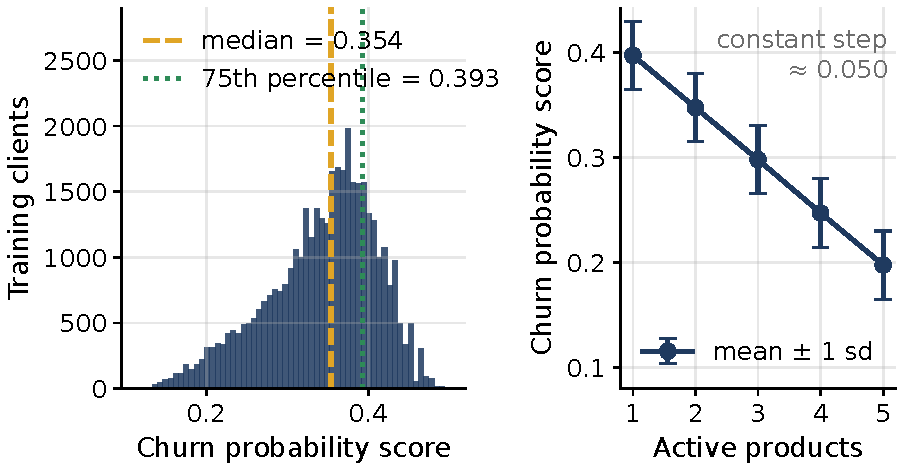
\includegraphics[width=\linewidth]{fig_target.pdf}
  \caption{Izquierda: distribución del puntaje \cp\ en el entrenamiento con los umbrales de la mediana
  (etiqueta de la entrega anterior) y del percentil 75 (etiqueta de este trabajo). Derecha: media y desviación
  del puntaje por número de productos activos; el paso constante delata la regla con la que se generó el
  puntaje y justifica excluir esa variable.}
  \label{fig:objetivo}
\end{figure}

\paragraph{Particiones y control de fugas.}
La partición es 80/20 por índices con semilla 42 ($n = 38.978$ clientes de entrenamiento y
$n_{\mathrm{te}} = 9.745$ de prueba),
aleatoria y no por posición porque el archivo está ordenado por cohortes, y se hace antes de calcular
cualquier estadístico del objetivo: el umbral $\tau$ se estima solo con el entrenamiento y la prueba no se
toca hasta la evaluación final. Se eligió la etiqueta del percentil 75 porque con la mediana las clases
quedan al 50~\% por construcción y el balanceo no tiene nada que hacer. Toda selección de hiperparámetros se
hace dentro del entrenamiento con validación cruzada anidada (sección~\ref{sec:entrenamiento}), y las
pruebas que dependen del orden de las filas se calculan en el orden original del archivo, que induce
dependencia entre vecinos.

\subsection{Modelo propuesto}
\label{sec:modelo}

\paragraph{Idea central.}
Se propone una \emph{Explainable Boosting Machine} (EBM) \citep{lou2012intelligible,lou2013ga2m}, en la
implementación \texttt{interpret} \citep{nori2019interpretml}: un modelo aditivo generalizado con
interacciones por pares (GA$^2$M) cuyas funciones de forma se aprenden por \emph{boosting} cíclico de árboles
de pocas hojas. Reúne dos propiedades que rara vez van juntas: la flexibilidad del \emph{boosting} para
representar efectos no lineales y la legibilidad de un modelo aditivo, en el que la predicción es
literalmente la suma de curvas que se pueden graficar y auditar. No forma parte de los modelos del curso. Para
adaptarla al problema se implementa la ponderación de clases mediante pesos por observación y se aplica una
búsqueda de hiperparámetros multi-fidelidad; la figura~\ref{fig:ebm} muestra la arquitectura.

\begin{figure}[tbp]
  \centering
  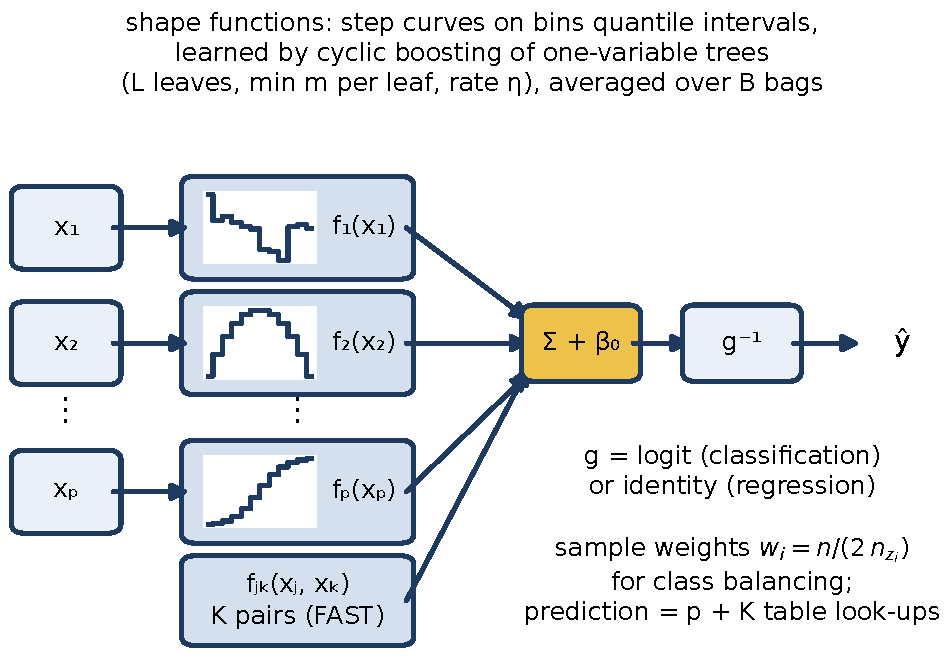
\includegraphics[width=\linewidth]{fig_ebm_architecture.pdf}
  \caption{Arquitectura del modelo propuesto: cada predictor aporta una función de forma escalonada, las
  $K$ interacciones por pares aportan una superficie cada una, la suma pasa por el enlace inverso y da la
  predicción. Cada función se aprende por \emph{boosting} cíclico de árboles de una variable y se promedia
  sobre $B$ bolsas externas.}
  \label{fig:ebm}
\end{figure}

\paragraph{Formulación.}
La EBM modela
\begin{equation}
  g\big(\E[\,y \mid \bm{x}\,]\big) = \beta_0 + \sum_{j=1}^{p} f_j(x_j) + \sum_{(j,k) \in \mathcal{I}} f_{jk}(x_j, x_k),
  \label{eq:ebm}
\end{equation}
donde $y$ es $z$ o $s$ según la tarea, $g$ es el enlace logit en clasificación y la identidad en regresión,
$f_j$ son funciones de forma unidimensionales y $\mathcal{I}$ es un conjunto de $K$ pares elegido con el
algoritmo FAST \citep{lou2013ga2m}. A diferencia de un GAM con \emph{splines}, cada $f_j$ es una función
escalonada sobre una discretización de $x_j$ en $\mathrm{bins}$ intervalos por cuantiles, aprendida por
\emph{boosting} cíclico: en cada ronda $r$ se recorren las $p$ variables en orden y, para cada una, se ajusta
un árbol de regresión $h$ de $L$ hojas y al menos $m$ observaciones por hoja \emph{solo sobre esa variable} al
gradiente negativo de la pérdida en la predicción acumulada $\hat{u}_i$ (en la escala de $g$), y se añade
escalado por una tasa $\eta$ pequeña:
\begin{equation}
  f_j^{(r+1)}(x_j) = f_j^{(r)}(x_j) + \eta\, h_j^{(r)}(x_j),
  \qquad
  h_j^{(r)} = \arg\min_{h} \sum_{i=1}^{n} w_i \big( \varrho_i^{(r)} - h(x_{ij}) \big)^2,
  \label{eq:boosting}
\end{equation}
con $\ell(y_i, \hat{u}_i)$ el término del cliente $i$ en la pérdida de la ecuación~\eqref{eq:perdidas}, escrito
en la escala del enlace ($\hat{u}_i = \operatorname{logit} \hat{p}_i$ en clasificación y $\hat{u}_i = \hat{s}_i$ en
regresión), y $\varrho_i^{(r)} = -\partial \ell(y_i, \hat{u}_i^{(r)}) / \partial \hat{u}_i^{(r)}$ su gradiente
negativo. La tasa baja hace que el orden de las variables no importe y reparte la señal compartida entre variables
correlacionadas. El procedimiento se repite sobre $B$ submuestras (bolsas externas) y las funciones se
promedian, $f_j = \frac{1}{B}\sum_b f_j^{(b)}$, lo que reduce su varianza y da un intervalo para cada tramo.
La predicción de un cliente es una suma de $p + K$ búsquedas en tablas.

\paragraph{Adaptaciones.}
La librería no ofrece ponderación de clases; se implementó un envoltorio que, cuando la corrida usa
ponderación, pasa a la EBM pesos por observación
\begin{equation}
  w_i = \frac{n}{2\, n_{z_i}},
  \label{eq:pesos}
\end{equation}
con $n_{z_i}$ el número de clientes de la clase de $i$, de modo que la pérdida ponderada
$\sum_i w_i\, \ell(y_i, \hat{u}_i)$ de la ecuación~\eqref{eq:perdidas} equivale a la ponderación balanceada de scikit-learn que reciben los modelos de
referencia. La búsqueda de hiperparámetros es multi-fidelidad: durante la búsqueda cada configuración se
evalúa con $B = 2$ bolsas y el modelo que se mide en el bucle externo y se guarda se reajusta con $B = 8$;
como las bolsas promedian pero no cambian la forma de cada función, el orden de las configuraciones se
conserva, supuesto que se comprueba empíricamente (sección~\ref{sec:ablacion}). El espacio de búsqueda es
$\eta \in [0{,}008;\ 0{,}1]$ (escala logarítmica; por debajo de 0,008 cada ajuste tarda el doble),
$L \in \{2, 3, 4\}$, $m \in [2, 200]$ (log), $K \in \{0, \dots, 20\}$ (0 es un GAM puro) y
$\mathrm{bins} \in [64, 1024]$ (log), con una rejilla de 36 puntos. El algoritmo~\ref{alg:ebm} resume el
entrenamiento.

\begin{algorithm}[t]
  \caption{Entrenamiento de la EBM con bolsas externas, pesos de clase y multi-fidelidad.}
  \label{alg:ebm}
  \begin{algorithmic}[1]
    \Require entrenamiento $\{(\bm{x}_i, y_i)\}_{i=1}^{n}$; pesos $w_i$ (1, o la ecuación~\eqref{eq:pesos} con ponderación); bolsas $B$; tasa $\eta$; hojas $L$; mínimo por hoja $m$; pares $K$; intervalos $\mathrm{bins}$
    \Ensure $\beta_0$, funciones de forma $f_j$ y $f_{jk}$
    \State discretizar cada $x_j$ en $\mathrm{bins}$ intervalos por cuantiles (una sola vez)
    \For{$b = 1, \dots, B$}
      \State tomar una submuestra de entrenamiento y reservar el resto como validación de la bolsa
      \State $f_j^{(b)} \gets 0$ para todo $j$;\quad $\hat{u}_i \gets \beta_0$ (logit de la media ponderada, o la media)
      \While{la pérdida ponderada en la validación de la bolsa mejore (parada temprana)}
        \For{$j = 1, \dots, p$} \Comment{ciclo sobre las variables}
          \State $\varrho_i \gets -\partial \ell(y_i, \hat{u}_i) / \partial \hat{u}_i$ para todo $i$
          \State ajustar un árbol $h$ de $L$ hojas y mínimo $m$ sobre $x_j$ al residuo $\varrho$ con pesos $w_i$
          \State $f_j^{(b)} \gets f_j^{(b)} + \eta\, h$;\quad $\hat{u}_i \gets \hat{u}_i + \eta\, h(x_{ij})$
        \EndFor
      \EndWhile
      \State elegir con FAST los $K$ pares $(j, k)$ que más reducen el residuo y repetir el ciclo sobre ellos con los $f_j^{(b)}$ fijos
    \EndFor
    \State $f_j \gets \frac{1}{B}\sum_b f_j^{(b)}$ y $f_{jk} \gets \frac{1}{B}\sum_b f_{jk}^{(b)}$, centradas;\quad $\beta_0 \gets$ media de las predicciones
    \State \textbf{búsqueda:} evaluar cada configuración con $B = 2$ en la validación interna; \textbf{modelo final:} reajustar la ganadora con $B = 8$
  \end{algorithmic}
\end{algorithm}

\paragraph{Justificación de cada componente.}
El análisis exploratorio muestra que la señal está en pocas variables con efectos no lineales y que los
pares de predictores son casi independientes: esa es exactamente la hipótesis aditiva de la
ecuación~\eqref{eq:ebm}, que representa escalones, mesetas y curvas en S sin interacciones profundas. Frente
a los modelos lineales, la EBM gana flexibilidad por variable; frente a XGBoost y Random Forest, restringe el
espacio de hipótesis a sumas de funciones de una variable y de pocos pares, lo que reduce la varianza en un
problema con 39.000 filas y una señal débil. Las bolsas externas estabilizan las curvas como el
\emph{bagging} de un bosque. Los pesos de la ecuación~\eqref{eq:pesos} ponen a la EBM en igualdad de
condiciones con las referencias cuando la corrida usa ponderación de clases, y la multi-fidelidad hace viable
una búsqueda cuyo coste crece con $B$. Finalmente, el modelo no necesita un explicador: cada $f_j$ es la
explicación.

\paragraph{Complejidad computacional.}
El entrenamiento recorre las $p$ variables en cada ronda: cuesta $O(B\, M\, p\, (n + \mathrm{bins}))$ para
$M$ rondas, con $n = 38.978$, $p = 78$ y $B = 8$ en el modelo final; la inferencia cuesta $O(p + K)$
búsquedas en tablas por cliente. Los parámetros del modelo son los valores de las funciones escalonadas: a
lo sumo $p \cdot \mathrm{bins}$ números para las funciones de una variable y $K \cdot \mathrm{bins}^2$ para
los pares; en el modelo final ($K = 0$, $\mathrm{bins} = 1024$) son a lo sumo $32 \cdot 1024 + 46 \cdot 2 \approx
32.900$ valores, porque las 46 columnas indicadoras y booleanas solo tienen dos intervalos, y el modelo
serializado ocupa 1,5~MB frente a los 44~MB de un bosque de 300 árboles. Medido en el equipo de la sección~\ref{sec:entrenamiento},
el ajuste final tarda 26,7~s en clasificación y 31,8~s en regresión, la inferencia sobre los 9.745 clientes
de prueba 0,067 y 0,054~s, y la corrida anidada completa 18,7 y 26,6 minutos.

\paragraph{Qué es nuevo y qué se reutiliza.}
Se reutilizan la EBM tal como la publican \citet{lou2013ga2m} y su implementación \texttt{interpret-core}
\citep{nori2019interpretml}, el conjunto de datos y las decisiones de depuración de las entregas anteriores
(columnas eliminadas y variables transaccionales derivadas), revalidadas aquí con la partición hecha antes de
cualquier estadístico del objetivo, y el pipeline combinatorio y el protocolo estadístico de la guía del curso. Lo nuevo es la
elección y la adaptación del modelo a este problema: no se vio en el curso, la ponderación de clases por
observación y la búsqueda multi-fidelidad no existen en la librería, y la EBM se integra en el mismo
pipeline, con las mismas reglas y el mismo presupuesto, que los modelos de referencia, de modo que la
comparación es justa.

\subsection{Entrenamiento y optimización}
\label{sec:entrenamiento}

\paragraph{Optimización.}
La EBM se ajusta por el \emph{boosting} cíclico del algoritmo~\ref{alg:ebm}, con parada temprana por bolsa
sobre su validación interna y sin lotes ni épocas en el sentido de las redes. No tiene penalización explícita:
la regularizan la tasa $\eta$ baja, el mínimo $m$ por hoja, las $L \leq 4$ hojas, la parada temprana y el
promedio sobre $B$ bolsas. Sus hiperparámetros finales, elegidos por el protocolo de la
sección~\ref{sec:protocolo}, aparecen en la tabla~\ref{tab:espacios}. Los
modelos de referencia usan el solucionador de su implementación: liblinear para la logística, Cholesky para
Ridge, descenso por coordenadas para Lasso, el método \texttt{hist} para XGBoost y el primal con pérdida de
bisagra al cuadrado para el SVM lineal, elegidos tras medir su coste.

\begin{table}[t]
  \centering\scriptsize\setlength{\tabcolsep}{3pt}
  \caption{Espacios de búsqueda (rejilla de Grid Search, igual al presupuesto de los otros tres métodos) e
  hiperparámetros finales de la mejor combinación en clasificación (Clas.) y en regresión (Regr.).}
  \label{tab:espacios}
  \begin{tabular}{@{}>{\raggedright\arraybackslash}p{0.13\linewidth} r >{\raggedright\arraybackslash}p{0.42\linewidth} >{\raggedright\arraybackslash}p{0.33\linewidth}@{}}
    \toprule
    Modelo & Rejilla & Espacio de búsqueda & Hiperparámetros finales \\
    \midrule
    EBM (propuesto) & 36 & $\eta \in [0{,}008;\ 0{,}1]$ (log); $L \in \{2, 3, 4\}$; $m \in [2, 200]$ (log); $K \in \{0, \dots, 20\}$; $\mathrm{bins} \in [64, 1024]$ (log) & Clas.: $K = 0$, $\eta = 0{,}008$, $L = 2$, $m = 100$, $B = 8$, $\mathrm{bins} = 1024$ (valor por defecto; la rejilla no lo recorre). Regr.: $K = 0$, $\eta = 0{,}008$, $L = 3$, $m = 20$, $B = 8$, $\mathrm{bins} = 1024$ \\
    k-NN & 32 & $k \in [5, 600]$ (entero, log); pesos uniformes o por distancia; $q \in \{1, 2\}$ & Clas.: $k = 600$, distancia, $q = 1$. Regr.: $k = 80$, distancia, $q = 1$ \\
    Naive Bayes & 30 & \texttt{var\_smoothing} $\in [10^{-11}, 10^{-3}]$ (log) & Clas.: $10^{-3}$ \\
    Regresión logística & 30 & $C \in [10^{-3}, 10^{2}]$ (log); penalización $\in \{\mathrm{L1}, \mathrm{L2}\}$ & Clas.: $C = 0{,}0563$, L1 \\
    Ridge / Lasso & 30 & $\alpha \in [10^{-3}, 10^{5}]$ / $[10^{-6}, 10^{-1}]$ (log) & Regr.: $\alpha = 613{,}9$ / $1{,}09 \cdot 10^{-4}$ \\
    Árbol de decisión & 48 & profundidad $\in [3, 30]$; mínimo por hoja $\in [1, 300]$ (log); $\gamma \in [10^{-6}, 10^{-2}]$ (Clas.) o $[10^{-8}, 10^{-4}]$ (Regr.) (log); Gini o entropía (Clas.) & Clas.: 22; 7; $3{,}9 \cdot 10^{-4}$; Gini. Regr.: 13; 101; $1{,}8 \cdot 10^{-6}$ \\
    Random Forest & 36 & profundidad $\in [4, 40]$; variables por partición $\in \{\sqrt{p}, \log_2 p, 0{,}3, 0{,}5\}$; mínimo por hoja $\in [1, 100]$ (log); $T = 100$ en la búsqueda y 300 en el final & Clas.: 32; 0,5; 11. Regr.: 8; 0,5; 50 \\
    XGBoost & 32 & árboles $\in [100, 1000]$ (log); profundidad $\in [2, 10]$; tasa $\in [10^{-3}, 0{,}3]$ (log); submuestreo de filas y de columnas $\in [0{,}5;\ 1]$; penalización L2 de las hojas $\lambda \in [0{,}01;\ 10]$ (log); peso mínimo por hoja $\in [1, 50]$ (log) & Clas.: 145; 6; 0,0033; 0,81; 0,97; 0,88; 11. Regr.: 512; 2; 0,024; 0,80; 0,73; 0,22; 31 \\
    SVM / SVR lineal & 30 & $C \in [10^{-4}, 10^{2}]$ (Clas.) o $[10^{-3}, 10^{2}]$ (Regr.) (log); $\varepsilon \in [10^{-4};\ 0{,}05]$ (log, Regr.) & Clas.: $C = 0{,}0011$. Regr.: $C = 46{,}4$, $\varepsilon = 3{,}8 \cdot 10^{-4}$ \\
    \bottomrule
  \end{tabular}
\end{table}

\paragraph{Búsqueda de hiperparámetros.}
Cada corrida es una validación cruzada anidada \citep{cawley2010overfitting}: un bucle externo de 5
pliegues (estratificados en clasificación, los mismos para todos los modelos) produce la única métrica que
se reporta, y dentro de cada pliegue externo un bucle interno de 3 pliegues elige los hiperparámetros con uno
de los cuatro métodos de la tabla~\ref{tab:optimizadores}, que reciben el mismo presupuesto: tantas
evaluaciones como puntos tiene la rejilla del modelo (entre 30 y 48). Al terminar, la misma búsqueda se
repite sobre todo el entrenamiento y el ganador se reajusta con él: es el modelo final, que toca la prueba
una sola vez. El mejor puntaje interno se guarda para medir el optimismo de selección, pero nunca se reporta.

\begin{table}[t]
  \centering\small
  \caption{Los cuatro métodos de búsqueda de hiperparámetros, con el mismo presupuesto por modelo.}
  \label{tab:optimizadores}
  \begin{tabular}{@{}>{\raggedright\arraybackslash}p{0.19\linewidth} >{\raggedright\arraybackslash}p{0.38\linewidth} >{\raggedright\arraybackslash}p{0.37\linewidth}@{}}
    \toprule
    Método & Cómo propone cada evaluación & Parámetros \\
    \midrule
    Grid Search & recorre la rejilla del modelo & puntos de la rejilla: de 30 a 48 \\
    Random Search & muestrea el espacio tipado & escala logarítmica para $C$, $\alpha$ y las tasas; enteros en escala logarítmica para vecinos y tamaños de hoja \\
    Bayesiana (TPE de Optuna \citep{akiba2019optuna}) & modela las densidades de las configuraciones mejores y del resto y propone el máximo de su cociente & 10 ensayos aleatorios de arranque; cuantil 0,10 para separar las mejores \\
    Genética (DEAP) & genes en $[0, 1]$, selección por torneo, cruce uniforme, mutación gaussiana y elitismo & torneo de 3; cruce con probabilidad 0,5 por gen, aplicado con 0,6; mutación con $\sigma = 0{,}15$ y probabilidad 1/(número de hiperparámetros) por gen, aplicada con 0,3; población entre 4 y 12 (presupuesto/4) \\
    \bottomrule
  \end{tabular}
\end{table}

\paragraph{Semillas, software y hardware.}
Una semilla única (42) se propaga a la partición, a cada estimador, al remuestreo, a los optimizadores y a
los \emph{bootstrap}; la sensibilidad a la semilla se mide reentrenando los modelos finales de Random
Forest, XGBoost, SVM y EBM con cinco a diez semillas y repitiendo la búsqueda del árbol con cinco semillas de
cada optimizador estocástico. El software es Python 3.13.3 con scikit-learn 1.9.1 \citep{pedregosa2011sklearn},
imbalanced-learn 0.14.2, XGBoost 3.4.1, interpret-core 0.7.8, Optuna 5.0.0 y DEAP 1.4.4, con las versiones
exactas fijadas. El equipo es un escritorio con procesador AMD de seis núcleos, 15,9~GB de memoria y una GPU
NVIDIA GeForce RTX~3050 de 6~GB (que no acelera estos modelos y solo se usó para medirlo), con Windows~11.
Las 140 corridas de la guía se ejecutaron en serie, con el equipo dedicado y el código congelado con su huella
SHA-256, y sumaron 26,9 horas; las 20 corridas de la EBM, 19,5 horas. El tiempo se reporta de tres formas:
duración de cada corrida anidada, ajuste del modelo final sobre los 38.978 clientes y tiempo de inferencia
sobre los 9.745 de prueba, estos dos como mediana de tres ajustes y cinco inferencias con el pipeline
completo.

\subsection{Modelos de referencia}
\label{sec:referencias}

\begin{sloppypar}
El modelo propuesto se compara con todos los modelos del curso en las dos tareas, en su implementación de
scikit-learn \citep{pedregosa2011sklearn} salvo XGBoost: k vecinos más cercanos, Naive
Bayes gaussiano, regresión logística con penalización L1 o L2, Ridge y Lasso,
árbol de decisión CART \citep{breiman1984cart}, Random Forest \citep{breiman2001rf}, XGBoost
\citep{chen2016xgboost} y máquinas de vectores de soporte lineales \citep{cortes1995svm}, porque el núcleo
RBF multiplica por 70 el coste del ajuste; se añaden los dos modelos de la entrega anterior, reentrenados con
sus hiperparámetros (regresión logística L1 con $C = 0{,}1$ y Lasso con $\alpha = 10^{-4}$). Todos usan las
mismas particiones, el mismo preprocesamiento y el mismo presupuesto de búsqueda que la EBM
(tabla~\ref{tab:espacios}), y cada clasificador se entrena con cuatro técnicas de balanceo: sin balanceo,
SMOTE \citep{chawla2002smote}, ADASYN y ponderación de clases con la ecuación~\eqref{eq:pesos}; el
sobremuestreo se ajusta solo con las filas de entrenamiento de cada pliegue y las combinaciones que no
aplican (k-NN con ponderación, que vota sin función de pérdida) se registran como tales. En regresión no hay
balanceo. Random Forest usa la misma multi-fidelidad que la EBM (100 árboles en la búsqueda, 300 en el modelo
final) y XGBoost pondera las clases con el cociente negativos/positivos del pliegue.
\end{sloppypar}

\subsection{Protocolo de evaluación}
\label{sec:protocolo}

\paragraph{Métricas.}
En clasificación, la métrica principal es el AUC; se reportan además el AUC-PR y, en el punto de operación
que contacta al 25~\% de clientes de mayor riesgo, la precisión, el \emph{recall}, el F1, el MCC y la exactitud
balanceada; el \emph{recall} con umbral 0,5 (la métrica secundaria de la entrega anterior) se usa para mostrar
el efecto del balanceo, y la calibración se mide con el error de calibración esperado antes y después de una
recalibración isotónica ajustada solo con predicciones fuera de pliegue. En regresión, la métrica principal es
el RMSE, con el MAE, el MAPE y el $R^2$, y los residuos se someten a las pruebas de White, BDS, Ljung-Box y de
normalidad. Las métricas principales de prueba (AUC; RMSE y $R^2$) llevan un intervalo \emph{bootstrap} BCa con
2.000 réplicas.

\paragraph{Validación.}
La validación cruzada anidada de la sección~\ref{sec:entrenamiento} produce, para cada corrida, la media y
la desviación de la métrica en los 5 pliegues externos, con las que se elige la mejor combinación de cada
modelo sin mirar la prueba, que se evalúa una sola vez con el modelo final (figura~\ref{fig:pipeline}). Como el objetivo se generó a partir de \ap, se estima además el
techo de información que deja su exclusión: el pronóstico de un oráculo (\emph{gradient boosting} de
histogramas) que sí la conoce, promediado sobre la distribución de \ap\ en el entrenamiento y evaluado en la
misma prueba.

\begin{figure}[tbp]
  \centering
  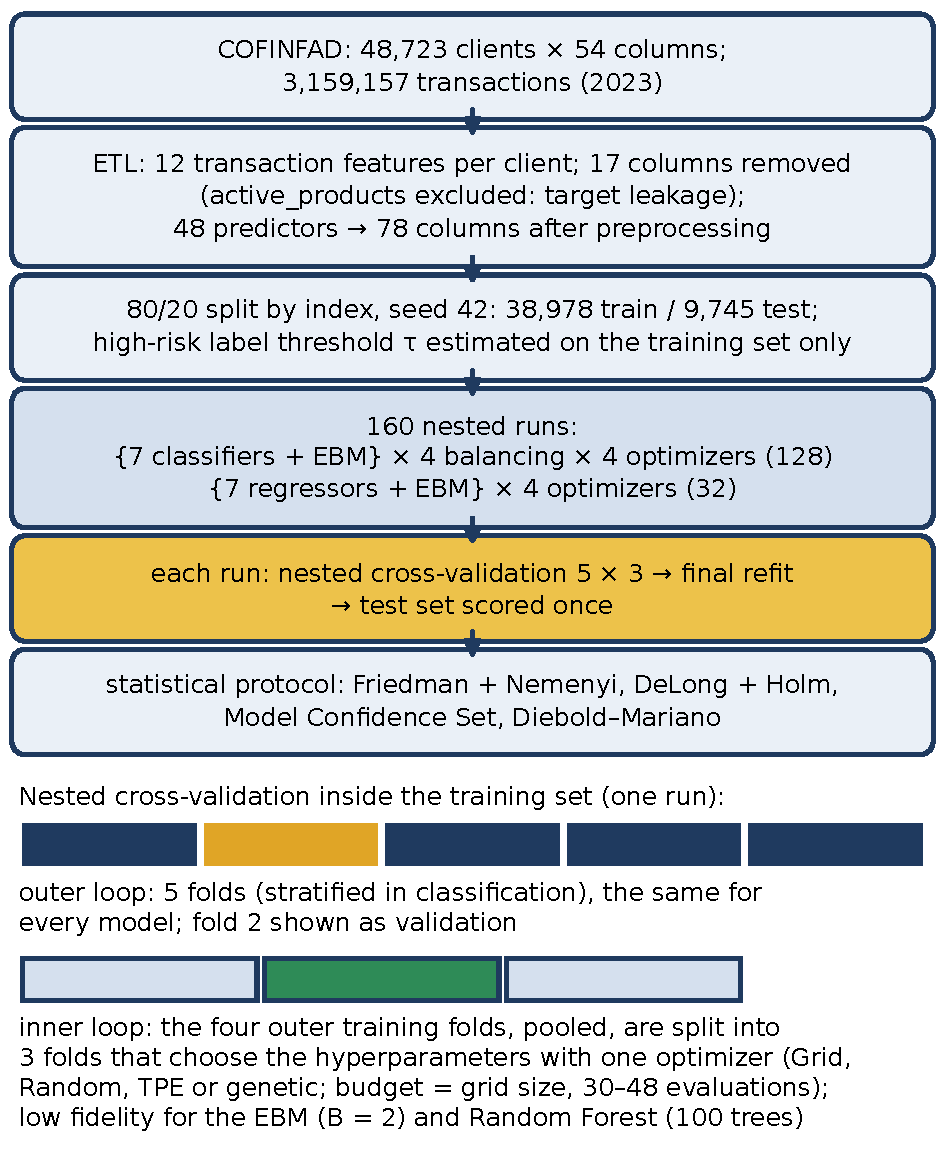
\includegraphics[width=\linewidth]{fig_pipeline_nested_cv.pdf}
  \caption{Pipeline combinatorio del estudio y validación cruzada anidada de cada corrida: el bucle externo
  de 5 pliegues produce la métrica que se reporta y el interno de 3 pliegues elige los hiperparámetros con
  uno de los cuatro optimizadores; el modelo final se reajusta con todo el entrenamiento y toca la prueba una
  sola vez.}
  \label{fig:pipeline}
\end{figure}

\paragraph{Pruebas estadísticas.}
El modelo propuesto se contrasta con cada uno de los siete modelos de referencia ($m = 7$) con $\alpha = 0{,}05$
y $p$ ajustados por Holm dentro de cada prueba. En clasificación: la $t$ pareada con varianza corregida de
\citet{nadeau2003} sobre los AUC de los 5 pliegues externos (los mismos para todos los modelos), DeLong
\citep{delong1988} sobre la prueba, McNemar exacta \citep{mcnemar1947}
sobre las clases del punto de operación y la $t$ correlacionada bayesiana \citep{benavoli2017} con una región de
equivalencia práctica de $\pm 0{,}01$ de AUC. En regresión: la $t$ corregida sobre el RMSE de los pliegues,
Diebold-Mariano \citep{diebold1995} con la corrección de Harvey-Leybourne-Newbold sobre las pérdidas cuadráticas
de la prueba, la bayesiana con región de $\pm 0{,}0005$ de RMSE y, como complemento, el \emph{Model Confidence
Set} al 90~\% \citep{hansen2011mcs} con \emph{bootstrap} estacionario, con las filas en el orden original del
archivo, organizado por bloques. Cada $p$ va con un tamaño de efecto: la diferencia de métrica con intervalo BCa,
la $d$ de Cohen y la delta de Cliff. La comparación con la entrega anterior se hace en su misma partición, su
misma etiqueta y su misma prueba, con la EBM y XGBoost afinados entre sí con el mismo procedimiento (TPE con
el presupuesto de la tabla~\ref{tab:espacios} y validación cruzada de 5 pliegues sobre el entrenamiento,
reajuste final y una sola evaluación en la prueba), y se decide con DeLong (clasificación) y Diebold-Mariano
(regresión). Los cuatro optimizadores se comparan con Friedman (Iman-Davenport) y Nemenyi \citep{demsar2006},
cuyos bloques son las combinaciones modelo $\times$ balanceo y no los pliegues de un solo conjunto, por la
métrica final y por el área bajo la curva de arrepentimiento normalizado de cada búsqueda.

\subsection{Diseño del estudio de ablación}
\label{sec:ablacion}

Cada variante cambia un solo componente del modelo propuesto y conserva el resto (particiones,
preprocesamiento, presupuesto y semilla). Hipótesis y diseño de cada variante:
\begin{enumerate}
  \item \textbf{Sin interacciones} ($K = 0$, un GAM puro) frente a la EBM con sus $K$ pares, en la
        partición y la etiqueta de la entrega anterior y decidido con DeLong sobre la prueba: la hipótesis
        aditiva basta porque la señal está en pocas variables casi independientes.
  \item \textbf{Balanceo} (sin balanceo, SMOTE, ADASYN y ponderación de clases) en las corridas anidadas de
        la EBM: no mejora el AUC, que mide el orden de los clientes, y solo desplaza el punto de operación.
  \item \textbf{Fidelidad de la búsqueda}: ocho configuraciones aleatorias evaluadas con $B = 2$ y con
        $B = 8$ en la misma validación cruzada de 3 pliegues ($\rho$ de Spearman entre ambos AUC, misma
        ganadora y ahorro de tiempo): la fidelidad baja conserva el orden y ahorra tiempo.
  \item \textbf{Optimizador} (Grid, Random, TPE y genético con el mismo presupuesto): la métrica final no
        distingue a los métodos; la eficiencia por evaluación (área de arrepentimiento, medida sobre las 140
        corridas de la guía) sí.
  \item \textbf{Semilla}: el modelo final de cada tarea se reentrena con cinco semillas (desviación de la
        métrica principal de prueba): la variabilidad por semilla es del orden de las diferencias entre los
        modelos de árboles.
\end{enumerate}

\subsection{Disponibilidad de código y datos}
\label{sec:disponibilidad}

COFINFAD es público y puede descargarse de Mendeley Data (DOI 10.17632/mhb4zn3258.1, licencia CC~BY~4.0);
una copia comprimida de las dos tablas está en la carpeta \texttt{datos} del repositorio y el código la
descomprime al cargarla. El código completo (paquete \texttt{src}, guiones de las corridas, de la comparación
con la entrega anterior y de los experimentos de cómputo), la tabla maestra con las 160 corridas, las
predicciones de prueba, los cuadernos ejecutados y el libro de Jupyter están en
\url{https://github.com/RubenEsg/Prediccion-de-fuga-de-clientes-en-fintech}; el entorno se fija con
\texttt{requirements.txt} (versiones exactas), la semilla es 42 y el hardware es el de la
sección~\ref{sec:entrenamiento}.

% Copia que genera armar.py desde resultados.tex de la carpeta de su sección; los cambios se hacen allí y se vuelve a armar.
% Sección de resultados del proyecto (Entregables 1 a 3). Se incluye desde main.tex. Toda cifra del texto, de las
% tablas y de las figuras la produce generar.py a partir de los resultados guardados del Entregable 3 (datos/*.csv).
\section{Resultados}
\label{sec:resultados}

Cada cifra de esta sección la reproduce un único guion, \texttt{generar.py}, desde los resultados guardados
del Entregable 3; guion, datos y figuras acompañan al código del proyecto en
\url{https://github.com/RubenEsg/Prediccion-de-fuga-de-clientes-en-fintech}.

\subsection{Resumen del montaje experimental}
\label{sec:montaje}

Los datos son los 48.723 clientes de COFINFAD \citep{cofinfad2025} con 48 predictores ($p = 78$ columnas),
partidos 80/20 con la semilla 42. En clasificación la etiqueta de riesgo alto es el cuarto
superior de \cp\ ($\tau = 0{,}3927$; 24,6~\% de positivos en la prueba). Cada modelo entra con su mejor
combinación según el bucle externo de la validación anidada $5 \times 3$ (mismos pliegues) y toca la prueba una
sola vez. La métrica principal es el AUC en clasificación y el RMSE en regresión; las secundarias, el AUC-PR, el
F1, el MCC y la exactitud balanceada con el 25~\% de capacidad de campaña, el ECE recalibrado, el MAE, el MAPE y
el $R^2$. El protocolo fija $\alpha = 0{,}05$ y Holm \citep{holm1979} sobre las siete comparaciones de cada
prueba. La métrica principal, $\alpha$, Holm, DeLong, Diebold-Mariano y el \emph{Model Confidence Set} se
fijaron en el Entregable 3 antes de evaluar la prueba; la $t$ corregida, McNemar, la bayesiana (con regiones de
equivalencia de $\pm 0{,}01$ de AUC y $\pm 0{,}0005$ de RMSE fijadas antes de ejecutarla) y los análisis de
sensibilidad son posteriores y exploratorios.

\subsection{Desempeño predictivo global}
\label{sec:global}

\paragraph{Clasificación.}
La tabla~\ref{tab:clasificacion} resume la prueba y la figura~\ref{fig:folds} los pliegues. En la prueba la EBM
obtiene el mayor AUC de los ocho modelos, 0,8289 con intervalo BCa [0,8206; 0,8366], seguida de XGBoost,
Random Forest y el árbol de decisión (0,8283 a 0,8243); después vienen k-NN (0,787), los lineales (0,771) y
Naive Bayes (0,666). En la validación anidada la EBM queda cuarta, a 0,0040 de XGBoost y del árbol, el orden
de la desviación entre pliegues. La misma estructura de tres grupos aparece en el AUC-PR (0,551) y en las
curvas ROC y precisión-\emph{recall} de la
figura~\ref{fig:roc_pr}. En el
punto de operación, en cambio, los siete modelos distintos de Naive Bayes son indistinguibles: contactando al
25~\% de mayor riesgo, la EBM captura el 51,2~\% de la fuga con una precisión del 50,4~\% (MCC 0,346) y la
regresión logística el 51,1~\% (MCC 0,344); la tabla~\ref{tab:confusion} da las matrices de confusión con esa
regla y con el umbral 0,5. Las probabilidades sin
recalibrar están sesgadas en los modelos con ponderación (ECE de 0,170 en la EBM); la recalibración isotónica
ajustada con predicciones fuera de pliegue lo deja entre 0,003 y 0,010 y apenas mueve el AUC
(figura~\ref{fig:calibration}). En resumen, por el valor puntual del AUC de prueba y del AUC-PR la EBM queda
por delante de las siete referencias, aunque solo cuatro ventajas son significativas
(sección~\ref{sec:pruebas}); la mayor es $+0{,}058$ de AUC frente a la logística ($+7{,}5$~\% relativo) y la
menor, $+0{,}0006$ frente a XGBoost; por el AUC externo gana cuatro y pierde tres, y en el punto de operación
empata con seis.

\paragraph{Regresión.}
Según la tabla~\ref{tab:regresion}, XGBoost tiene el menor RMSE de prueba (0,05917) y la EBM el segundo
(0,05925), con Random Forest y el árbol dentro de los mismos intervalos; los lineales quedan un 4~\% por encima
y k-NN un 7~\%. El $R^2$ pasa de 0,151 en Ridge y Lasso a 0,216 en la EBM y 0,218 en XGBoost, y el MAPE, de
17,1 a 16,0~\%: la EBM pierde con XGBoost en las cuatro métricas por milésimas o menos y gana a los otros seis.
El pronóstico sigue la tendencia pero
se comprime hacia la media (figura~\ref{fig:regression}), y el residuo de la EBM es asimétrico (asimetría
$-0{,}90$) y no normal, sin heterocedasticidad (White, $p = 0{,}67$) ni dependencia en el orden del archivo
(Ljung-Box, $p = 0{,}81$), según el diagnóstico del Entregable 3; la causa se identifica en la
sección~\ref{sec:errores}.

\paragraph{Frente a la entrega anterior.}
En su partición y etiqueta de la mediana (tabla~\ref{tab:entrega2}), la EBM sube el AUC de la logística L1 de
0,6832 a 0,7187 y baja el RMSE del Lasso de 0,06166 a 0,05926 ($p$ ajustado $< 0{,}001$ en DeLong y en
Diebold-Mariano); frente a XGBoost queda a $-0{,}0019$ de AUC ($p = 0{,}20$) y a $0{,}00007$ de RMSE
($p = 0{,}07$).

\begin{table}[tbp]
  \centering\scriptsize\setlength{\tabcolsep}{3pt}
  \caption{Clasificación (riesgo alto = percentil 75): mejor combinación de cada modelo según el bucle externo. AUC externa (media $\pm$ desviación de los 5 pliegues), AUC de prueba con intervalo \emph{bootstrap} BCa al 95~\%, AUC-PR y, en el punto de operación que contacta al 25~\% de mayor riesgo, F1, MCC y exactitud balanceada; ECE tras la recalibración isotónica. Las métricas secundarias son valores puntuales de la prueba; el \emph{recall} y la precisión de ese punto están en la tabla~\ref{tab:confusion}. Negrita: mejor; subrayado: segundo (los empates comparten la marca). $^{\dagger}$: difiere de la EBM en DeLong tras Holm; $^{\ddagger}$: en la $t$ corregida tras Holm.}
  \label{tab:clasificacion}
  \begin{tabular}{@{}l c c c c c c c@{}}
    \toprule
    Modelo & AUC externa & AUC prueba [IC 95~\%] & AUC-PR & F1$_{25}$ & MCC$_{25}$ & Ex. bal.$_{25}$ & ECE \\
    \midrule
    \textbf{EBM (propuesto)} & $0{,}8292$ $\pm$ $0{,}0037$ & {\boldmath\textbf{$0{,}8289$ [$0{,}8206$; $0{,}8366$]}} & {\boldmath\textbf{$0{,}551$}} & {\boldmath\textbf{$0{,}508$}} & {\boldmath\textbf{$0{,}346$}} & {\boldmath\textbf{$0{,}674$}} & $0{,}006$ \\
    XGBoost & {\boldmath\textbf{$0{,}8332$ $\pm$ $0{,}0049$}} & \underline{$0{,}8283$ [$0{,}8203$; $0{,}8359$]} & \underline{$0{,}548$} & $0{,}506$ & $0{,}343$ & \underline{$0{,}673$} & $0{,}007$ \\
    Random Forest & \underline{$0{,}8326$ $\pm$ $0{,}0029$} & $0{,}8260$ [$0{,}8184$; $0{,}8338$] & $0{,}544$ & $0{,}490$ & $0{,}321$ & $0{,}662$ & {\boldmath\textbf{$0{,}003$}} \\
    Árbol de decisión & {\boldmath\textbf{$0{,}8332$ $\pm$ $0{,}0021$}} & $0{,}8243$ [$0{,}8165$; $0{,}8319$] & $0{,}530$ & $0{,}498$ & $0{,}333$ & $0{,}667$ & $0{,}010$ \\
    k-NN$^{\dagger\ddagger}$ & $0{,}7836$ $\pm$ $0{,}0072$ & $0{,}7874$ [$0{,}7777$; $0{,}7966$] & $0{,}502$ & $0{,}504$ & $0{,}341$ & $0{,}671$ & $0{,}008$ \\
    Regresión logística$^{\dagger\ddagger}$ & $0{,}7644$ $\pm$ $0{,}0047$ & $0{,}7709$ [$0{,}7600$; $0{,}7806$] & $0{,}508$ & \underline{$0{,}507$} & \underline{$0{,}344$} & \underline{$0{,}673$} & $0{,}006$ \\
    SVM lineal$^{\dagger\ddagger}$ & $0{,}7641$ $\pm$ $0{,}0044$ & $0{,}7706$ [$0{,}7599$; $0{,}7803$] & $0{,}507$ & \underline{$0{,}507$} & \underline{$0{,}344$} & \underline{$0{,}673$} & $0{,}007$ \\
    Naive Bayes$^{\dagger\ddagger}$ & $0{,}6722$ $\pm$ $0{,}0119$ & $0{,}6662$ [$0{,}6537$; $0{,}6787$] & $0{,}363$ & $0{,}405$ & $0{,}209$ & $0{,}605$ & \underline{$0{,}004$} \\
    \bottomrule
  \end{tabular}
\end{table}

\begin{table}[tbp]
  \centering\small\setlength{\tabcolsep}{3pt}
  \caption{Matrices de confusión en la prueba (9.745 clientes, 2.399 de riesgo alto) de la EBM y de XGBoost con la regla de decisión de la campaña (se contacta al 25~\% de mayor puntaje, 2.436 clientes) y con el umbral 0,5 de probabilidad: verdaderos positivos (VP), falsos positivos (FP), falsos negativos (FN), verdaderos negativos (VN), precisión y \emph{recall}.}
  \label{tab:confusion}
  \begin{tabular}{@{}l l r r r r c c@{}}
    \toprule
    Regla & Modelo & VP & FP & FN & VN & Precisión & Recall \\
    \midrule
    25~\% de mayor riesgo & \textbf{EBM (propuesto)} & 1.228 & 1.208 & 1.171 & 6.138 & $0{,}504$ & $0{,}512$ \\
    25~\% de mayor riesgo & XGBoost & 1.224 & 1.212 & 1.175 & 6.134 & $0{,}502$ & $0{,}510$ \\
    \midrule
    umbral 0,5 & \textbf{EBM (propuesto)} & 1.697 & 1.928 & 702 & 5.418 & $0{,}468$ & $0{,}707$ \\
    umbral 0,5 & XGBoost & 2.395 & 2.956 & 4 & 4.390 & $0{,}448$ & $0{,}998$ \\
    \bottomrule
  \end{tabular}
\end{table}

\begin{table}[tbp]
  \centering\scriptsize\setlength{\tabcolsep}{1.5pt}
  \caption{Regresión de \cp: mejor optimizador de cada modelo según el bucle externo. RMSE externo (media $\pm$ desviación de los 5 pliegues), RMSE de prueba con intervalo BCa al 95~\%, MAE, MAPE y $R^2$ con intervalo BCa, y $p$-valor del \emph{Model Confidence Set} al 90~\% (pertenecen al conjunto los modelos con $p > 0{,}10$). Negrita: mejor; subrayado: segundo. $^{\dagger}$: difiere de la EBM en Diebold-Mariano tras Holm; $^{\ddagger}$: en la $t$ corregida tras Holm.}
  \label{tab:regresion}
  \begin{tabular}{@{}l c c c c c c@{}}
    \toprule
    Modelo & RMSE externo & RMSE prueba [IC 95~\%] & MAE & MAPE & $R^2$ [IC 95~\%] & $p$ MCS \\
    \midrule
    XGBoost & {\boldmath\textbf{$0{,}05898$ $\pm$ $0{,}00040$}} & {\boldmath\textbf{$0{,}05917$ [$0{,}05841$; $0{,}06002$]}} & {\boldmath\textbf{$0{,}0471$}} & {\boldmath\textbf{$15{,}98$~\%}} & {\boldmath\textbf{$0{,}218$ [$0{,}203$; $0{,}232$]}} & $1{,}000$ \\
    \textbf{EBM (propuesto)} & \underline{$0{,}05903$ $\pm$ $0{,}00043$} & \underline{$0{,}05925$ [$0{,}05849$; $0{,}06009$]} & \underline{$0{,}0472$} & \underline{$16{,}03$~\%} & \underline{$0{,}216$ [$0{,}201$; $0{,}230$]} & $0{,}072$ \\
    Random Forest & $0{,}05915$ $\pm$ $0{,}00039$ & $0{,}05931$ [$0{,}05854$; $0{,}06013$] & $0{,}0473$ & $16{,}05$~\% & $0{,}215$ [$0{,}200$; $0{,}228$] & $0{,}006$ \\
    Árbol de decisión & $0{,}05926$ $\pm$ $0{,}00038$ & $0{,}05944$ [$0{,}05864$; $0{,}06025$] & $0{,}0475$ & $16{,}11$~\% & $0{,}211$ [$0{,}196$; $0{,}225$] & $<0{,}001$ \\
    Lasso$^{\dagger\ddagger}$ & $0{,}06180$ $\pm$ $0{,}00048$ & $0{,}06166$ [$0{,}06082$; $0{,}06251$] & $0{,}0507$ & $17{,}10$~\% & $0{,}151$ [$0{,}138$; $0{,}164$] & $<0{,}001$ \\
    Ridge$^{\dagger\ddagger}$ & $0{,}06182$ $\pm$ $0{,}00048$ & $0{,}06167$ [$0{,}06082$; $0{,}06252$] & $0{,}0507$ & $17{,}10$~\% & $0{,}151$ [$0{,}138$; $0{,}164$] & $<0{,}001$ \\
    SVR lineal$^{\dagger\ddagger}$ & $0{,}06183$ $\pm$ $0{,}00047$ & $0{,}06170$ [$0{,}06087$; $0{,}06255$] & $0{,}0507$ & $17{,}10$~\% & $0{,}150$ [$0{,}137$; $0{,}163$] & $<0{,}001$ \\
    k-NN$^{\dagger\ddagger}$ & $0{,}06335$ $\pm$ $0{,}00042$ & $0{,}06321$ [$0{,}06238$; $0{,}06409$] & $0{,}0511$ & $17{,}28$~\% & $0{,}108$ [$0{,}101$; $0{,}115$] & $<0{,}001$ \\
    \bottomrule
  \end{tabular}
\end{table}

\begin{table}[tbp]
  \centering\scriptsize\setlength{\tabcolsep}{2pt}
  \caption{Comparación con los modelos de la entrega anterior (E2) en su misma partición, etiqueta (mediana estimada con el entrenamiento) y prueba, tal como la calculó el Entregable 3. Clasificación: AUC con intervalo BCa, \emph{recall} con umbral 0,5, mejora de AUC frente a la logística L1 con intervalo BCa, $z$ de DeLong y $p$ ajustado por Holm, delta de Cliff sobre los 5 pliegues. Regresión: RMSE con intervalo BCa, $R^2$, reducción del RMSE frente al Lasso con intervalo BCa, Diebold-Mariano (HLN) y $p$ ajustado, delta de Cliff entre pliegues.}
  \label{tab:entrega2}
  \begin{tabular}{@{}l c c c c c@{}}
    \toprule
    Modelo & AUC o RMSE [IC 95~\%] & Recall$_{0{,}5}$ o $R^2$ & Mejora vs.\ E2 [IC 95~\%] & $z$ o DM; $p$ & $\delta$ \\
    \midrule
    Logística L1 (E2) & $0{,}6832$ [$0{,}6725$; $0{,}6931$] & $0{,}6515$ & -- & -- & -- \\
    XGBoost & $0{,}7206$ [$0{,}7107$; $0{,}7302$] & $0{,}6375$ & $+0{,}0374$ [$0{,}0303$; $0{,}0449$] & $10{,}06$; $2{,}5 \times 10^{-23}$ & $+1{,}00$ \\
    \textbf{EBM (propuesto)} & $0{,}7187$ [$0{,}7084$; $0{,}7284$] & $0{,}6565$ & $+0{,}0355$ [$0{,}0281$; $0{,}0434$] & $9{,}02$; $3{,}8 \times 10^{-19}$ & $+1{,}00$ \\
    \midrule
    Lasso (E2) & $0{,}06166$ [$0{,}06082$; $0{,}06251$] & $0{,}1511$ & -- & -- & -- \\
    XGBoost & $0{,}05919$ [$0{,}05843$; $0{,}06004$] & $0{,}2177$ & $+0{,}00247$ [$0{,}00210$; $0{,}00279$] & $14{,}05$; $5{,}9 \times 10^{-44}$ & $+1{,}00$ \\
    \textbf{EBM (propuesto)} & $0{,}05926$ [$0{,}05849$; $0{,}06010$] & $0{,}2159$ & $+0{,}00240$ [$0{,}00205$; $0{,}00274$] & $13{,}33$; $7{,}1 \times 10^{-40}$ & $+1{,}00$ \\
    \bottomrule
  \end{tabular}
\end{table}


\begin{figure}[tbp]
  \centering
  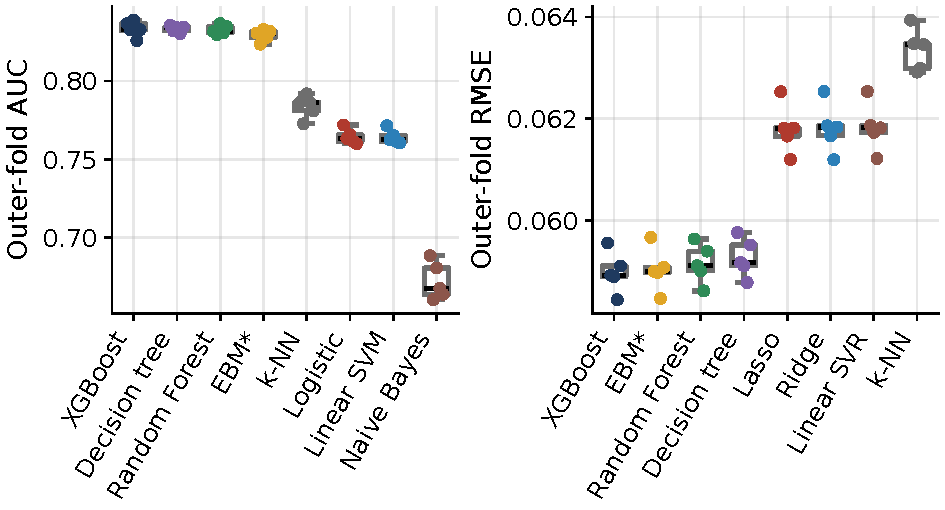
\includegraphics[width=\linewidth]{fig_folds.pdf}
  \caption{Métrica principal en cada uno de los 5 pliegues externos (puntos) y su diagrama de caja (mediana y
  cuartiles; bigotes hasta el mínimo y el máximo) para la mejor combinación de cada modelo: AUC en clasificación
  (izquierda) y RMSE en regresión (derecha). El asterisco marca el modelo propuesto.}
  \label{fig:folds}
\end{figure}

\begin{figure}[tbp]
  \centering
  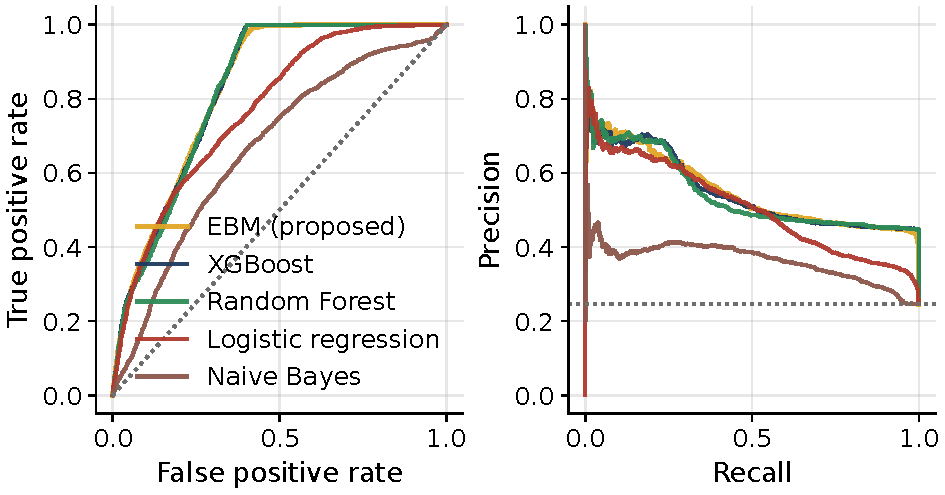
\includegraphics[width=\linewidth]{fig_roc_pr.pdf}
  \caption{Curvas ROC (izquierda) y precisión-\emph{recall} (derecha) en la prueba para la EBM, XGBoost, Random
  Forest, la regresión logística y Naive Bayes; la línea punteada es el azar (en precisión-\emph{recall}, la
  prevalencia de 0,246).}
  \label{fig:roc_pr}
\end{figure}

\begin{figure}[tbp]
  \centering
  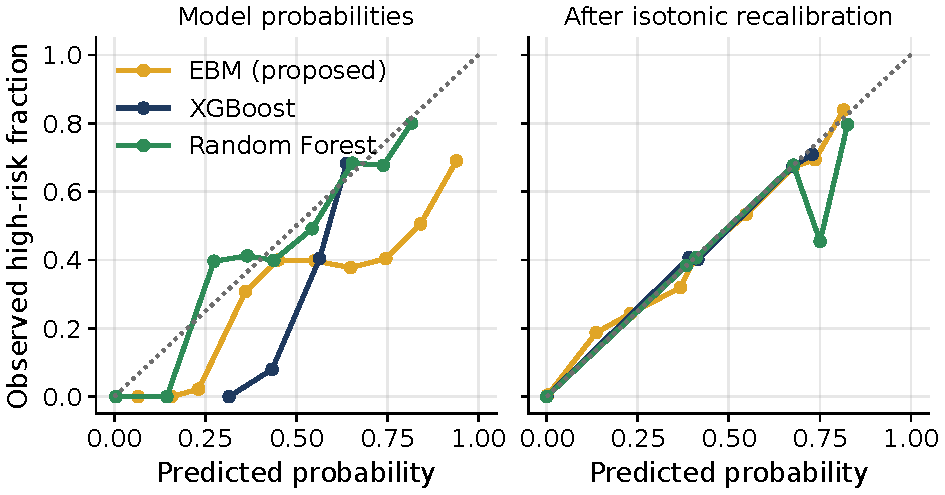
\includegraphics[width=\linewidth]{fig_calibration.pdf}
  \caption{Diagramas de confiabilidad en la prueba (10 intervalos de probabilidad) de la EBM, XGBoost y Random
  Forest antes (izquierda) y después (derecha) de la recalibración isotónica ajustada con predicciones fuera de
  pliegue del entrenamiento; la diagonal punteada es la calibración perfecta.}
  \label{fig:calibration}
\end{figure}

\begin{figure}[tbp]
  \centering
  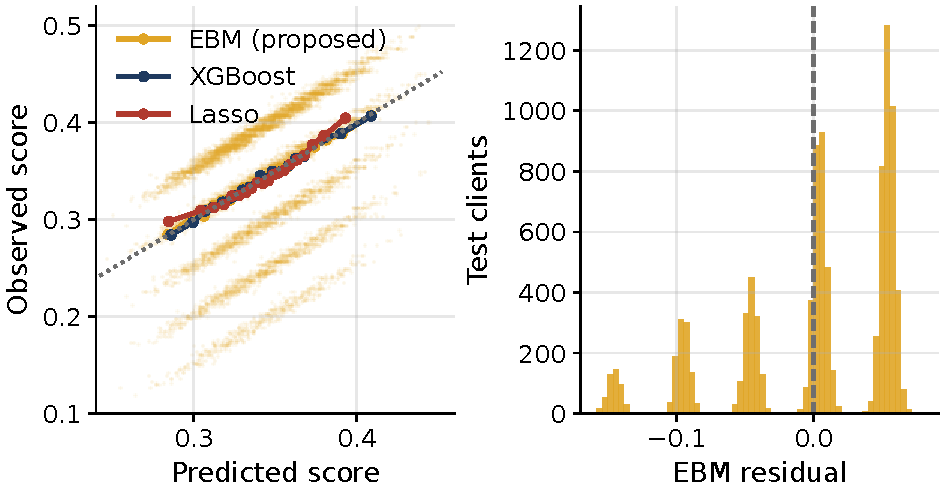
\includegraphics[width=\linewidth]{fig_regression.pdf}
  \caption{Regresión en la prueba. Izquierda: puntaje observado frente al pronóstico de la EBM (puntos,
  un cliente cada uno) y valor observado medio frente al pronóstico medio en 20 grupos de igual tamaño ordenados
  por el pronóstico para la EBM, XGBoost y Lasso (líneas); la diagonal punteada es la calibración perfecta.
  Derecha: distribución del residuo de la EBM (observado $-$ pronóstico).}
  \label{fig:regression}
\end{figure}

\subsection{Resultados de las pruebas de significancia}
\label{sec:pruebas}

Las tablas~\ref{tab:pruebas_clasificacion} a~\ref{tab:efectos_regresion} recogen, para cada modelo de
referencia, las pruebas, la diferencia con la EBM con su intervalo BCa de 2.000 réplicas y los tamaños de
efecto (figura~\ref{fig:intervals}). En
clasificación se aplican la $t$ pareada con varianza corregida de \citet{nadeau2003} sobre los AUC de los
cinco pliegues externos, DeLong \citep{delong1988} sobre la prueba, McNemar exacta \citep{mcnemar1947} sobre
las clases del punto de operación y la $t$ correlacionada bayesiana con región de equivalencia práctica
\citep{corani2015,benavoli2017}; en regresión, la $t$ corregida sobre el RMSE de los pliegues, Diebold-Mariano
con la corrección de \citet{harvey1997} sobre las pérdidas cuadráticas de la prueba, la bayesiana y, como
complemento, el \emph{Model Confidence Set} al 90~\% \citep{hansen2011mcs} con \emph{bootstrap} estacionario
\citep{politis1994}. Con cinco pliegues Wilcoxon no puede rechazar ($p$ mínimo 0,0625); se reporta la delta
de Cliff.

\paragraph{Clasificación.}
Frente a los cuatro modelos sin árboles la evidencia de diferencia es unánime: la $t$ corregida da
estadísticos de 14,3 a 23,2 y DeLong de 12,5 a 27,8, todos con $p$ ajustado menor que 0,001; los intervalos
de $\Delta$AUC quedan lejos de cero (de $+0{,}042$ a $+0{,}163$); la probabilidad posterior de que la EBM sea
mejor es mayor que 0,999, y el delta de Cliff es $+1$: la EBM gana en los cinco pliegues. Frente a XGBoost,
Random Forest y el árbol ninguna prueba rechaza: la $t$ corregida ($p$ ajustado de 0,16 a 0,25), DeLong ($p$
ajustado de 0,62 a 0,85) y los intervalos de $\Delta$AUC ($-0{,}006$ a $+0{,}012$) incluyen al cero; los signos
opuestos de las dos pruebas (unas milésimas por debajo en los pliegues, por encima en la prueba) son
variabilidad entre pliegues. El modelo
propuesto supera significativamente a 4 de 7 referencias; frente a las otras 3 ninguna prueba encuentra
evidencia de diferencia y la probabilidad de equivalencia práctica es 0,94 con XGBoost, 0,98 con el árbol y
0,997 con Random Forest, de modo que solo las dos últimas superan el umbral habitual del 95~\%.

McNemar discrepa, y la razón es informativa: sobre las clases del punto de operación solo separa a Naive
Bayes ($p < 0{,}001$); frente a k-NN y a los lineales el $p$ ajustado es 1,0, porque con la capacidad fija del
25~\% las tasas de error son 0,245--0,246 y 0,244 (la EBM identifica 1.228 clientes de riesgo alto de 2.399 y
la logística 1.225). La diferencia de AUC está en el resto de la curva ROC (figura~\ref{fig:roc_pr}),
es decir, en otras capacidades: con el 10~\% la EBM y la logística capturan el 25,6 y el 25,3~\% de la fuga,
pero con el 50~\% capturan el 91,2 y el 76,7~\%. La ventaja sobre un modelo lineal es real y crece con la
capacidad, pero en el punto de operación elegido vale tres clientes de cada 2.399: significancia estadística no
es relevancia práctica.

\paragraph{Regresión.}
Frente a los tres modelos lineales (Lasso, Ridge y SVR) y a k-NN la EBM reduce el RMSE en $0{,}0024$ a
$0{,}0040$ (intervalos que no incluyen el cero), con $t$ corregida de 27,9 a 63,3 y Diebold-Mariano de 13,3
a 17,5 ($p$ ajustado menor que 0,001), probabilidad bayesiana de ser mejor igual a 1, delta de Cliff $+1$ y
$d_z$ entre pliegues de 18,7 a 42,5; la $d_z$ por cliente (0,135 a 0,177) es pequeña: la mejora por cliente es
menor que el ruido de su pérdida, pero se repite en todos. Frente a XGBoost ($\Delta$RMSE $-0{,}00008$
[$-0{,}00016$; $+0{,}00001$]) ni la $t$ corregida ($p$ ajustado 0,43) ni Diebold-Mariano ($p$ ajustado 0,13)
rechazan, y la probabilidad de equivalencia dentro de $\pm 0{,}0005$ es 0,9998; tampoco rechazan frente a
Random Forest ($p$ ajustado 0,41). Frente al árbol las
pruebas discrepan: el intervalo de $\Delta$RMSE excluye al cero y Diebold-Mariano rechaza sin corregir
($p = 0{,}029$), pero no tras Holm ($p = 0{,}086$) ni en los pliegues ($p = 0{,}22$). El \emph{Model
Confidence Set} es más exigente: con 9.745 pérdidas correlacionadas y bloques de longitud 3 deja a XGBoost
como único miembro al 90~\%, y la EBM es la última en salir ($p_{\mathrm{MCS}} = 0{,}072$): hay una ventaja
sistemática de XGBoost de décimas de milésima (0,1~\%) que un procedimiento al 10~\% detecta y que ninguna
prueba al 5~\% con corrección confirma. En regresión el modelo propuesto supera significativamente a 4 de 7
referencias y es prácticamente equivalente a las otras 3.

\begin{table}[tbp]
  \centering\small\setlength{\tabcolsep}{3pt}
  \caption{Clasificación: pruebas de la EBM frente a cada modelo de referencia. $t$ corregida de Nadeau--Bengio sobre los AUC de los 5 pliegues externos (positiva cuando la EBM supera a la referencia); $z$ de DeLong sobre la prueba; McNemar exacta sobre las clases del punto de operación ($b$: clientes que solo la referencia clasifica bien; $c$: solo la EBM). Los $p$ son bilaterales y están ajustados por Holm sobre las siete comparaciones de cada prueba; los tamaños de efecto están en la tabla~\ref{tab:efectos_clasificacion}.}
  \label{tab:pruebas_clasificacion}
  \begin{tabular}{@{}l c c c@{}}
    \toprule
    Referencia & $t$ corr.; $p$ & DeLong $z$; $p$ & McNemar $b$/$c$; $p$ \\
    \midrule
    XGBoost & $-1{,}36$; $0{,}245$ & $0{,}19$; $0{,}848$ & 823/831; $1{,}000$ \\
    Random Forest & $-2{,}72$; $0{,}160$ & $0{,}90$; $0{,}737$ & 866/954; $0{,}248$ \\
    Árbol de decisión & $-2{,}07$; $0{,}215$ & $1{,}26$; $0{,}620$ & 1.106/1.152; $1{,}000$ \\
    k-NN & $14{,}32$; $5{,}5 \times 10^{-4}$ & $12{,}52$; $2{,}4 \times 10^{-35}$ & 728/746; $1{,}000$ \\
    Regresión logística & $18{,}12$; $2{,}7 \times 10^{-4}$ & $16{,}17$; $4{,}2 \times 10^{-58}$ & 730/736; $1{,}000$ \\
    SVM lineal & $19{,}88$; $2{,}3 \times 10^{-4}$ & $16{,}26$; $1{,}1 \times 10^{-58}$ & 727/733; $1{,}000$ \\
    Naive Bayes & $23{,}20$; $1{,}4 \times 10^{-4}$ & $27{,}78$; $5{,}4 \times 10^{-169}$ & 865/1.363; $2{,}8 \times 10^{-25}$ \\
    \bottomrule
  \end{tabular}
\end{table}

\begin{table}[tbp]
  \centering\small\setlength{\tabcolsep}{3pt}
  \caption{Clasificación: tamaños de efecto de la EBM frente a cada referencia. $\Delta$AUC $=$ AUC$_{\mathrm{EBM}} - $AUC$_{\mathrm{ref}}$ en la prueba con intervalo \emph{bootstrap} BCa al 95~\%; probabilidad posterior de la $t$ correlacionada bayesiana de que la EBM sea peor ($-$) / equivalente (ROPE $\pm 0{,}01$) / mejor ($+$); $d_z$ de Cohen y delta de Cliff (no pareada) entre pliegues, positivos cuando la EBM supera a la referencia.}
  \label{tab:efectos_clasificacion}
  \begin{tabular}{@{}l c c c c@{}}
    \toprule
    Referencia & $\Delta$AUC [IC 95~\%] & Bayes $-$ / ROPE / $+$ & $d_z$ & $\delta$ \\
    \midrule
    XGBoost & $+0{,}0006$ [$-0{,}0057$; $0{,}0071$] & $0{,}06$ / $0{,}94$ / $0{,}00$ & $-0{,}91$ & $-0{,}52$ \\
    Random Forest & $+0{,}0029$ [$-0{,}0035$; $0{,}0093$] & $0{,}00$ / $1{,}00$ / $0{,}00$ & $-1{,}82$ & $-0{,}44$ \\
    Árbol de decisión & $+0{,}0046$ [$-0{,}0019$; $0{,}0116$] & $0{,}02$ / $0{,}98$ / $0{,}00$ & $-1{,}39$ & $-0{,}68$ \\
    k-NN & $+0{,}0416$ [$0{,}0351$; $0{,}0479$] & $0{,}00$ / $0{,}00$ / $1{,}00$ & $9{,}61$ & $+1{,}00$ \\
    Regresión logística & $+0{,}0581$ [$0{,}0508$; $0{,}0651$] & $0{,}00$ / $0{,}00$ / $1{,}00$ & $12{,}15$ & $+1{,}00$ \\
    SVM lineal & $+0{,}0583$ [$0{,}0512$; $0{,}0654$] & $0{,}00$ / $0{,}00$ / $1{,}00$ & $13{,}34$ & $+1{,}00$ \\
    Naive Bayes & $+0{,}1627$ [$0{,}1510$; $0{,}1744$] & $0{,}00$ / $0{,}00$ / $1{,}00$ & $15{,}57$ & $+1{,}00$ \\
    \bottomrule
  \end{tabular}
\end{table}

\begin{table}[tbp]
  \centering\small\setlength{\tabcolsep}{3pt}
  \caption{Regresión: pruebas de la EBM frente a cada modelo de referencia. $t$ corregida sobre el RMSE de los 5 pliegues (positiva cuando la EBM pierde menos); Diebold-Mariano con la corrección HLN sobre las pérdidas cuadráticas de la prueba; $p$ del \emph{Model Confidence Set} al 90~\% de la referencia. Los $p$ de las dos primeras son bilaterales y están ajustados por Holm sobre las siete comparaciones; los tamaños de efecto están en la tabla~\ref{tab:efectos_regresion}.}
  \label{tab:pruebas_regresion}
  \begin{tabular}{@{}l c c c@{}}
    \toprule
    Referencia & $t$ corr.; $p$ & DM-HLN; $p$ & $p$ MCS \\
    \midrule
    XGBoost & $-1{,}48$; $0{,}428$ & $-1{,}85$; $0{,}128$ & $1{,}000$ \\
    Random Forest & $1{,}31$; $0{,}428$ & $0{,}82$; $0{,}410$ & $0{,}006$ \\
    Árbol de decisión & $2{,}41$; $0{,}221$ & $2{,}19$; $0{,}086$ & $<0{,}001$ \\
    Lasso & $57{,}21$; $3{,}4 \times 10^{-6}$ & $13{,}34$; $1{,}2 \times 10^{-39}$ & $<0{,}001$ \\
    Ridge & $51{,}33$; $4{,}3 \times 10^{-6}$ & $13{,}53$; $1{,}3 \times 10^{-40}$ & $<0{,}001$ \\
    SVR lineal & $63{,}28$; $2{,}6 \times 10^{-6}$ & $13{,}67$; $2{,}4 \times 10^{-41}$ & $<0{,}001$ \\
    k-NN & $27{,}88$; $3{,}9 \times 10^{-5}$ & $17{,}48$; $1{,}6 \times 10^{-66}$ & $<0{,}001$ \\
    \bottomrule
  \end{tabular}
\end{table}

\begin{table}[tbp]
  \centering\small\setlength{\tabcolsep}{3pt}
  \caption{Regresión: tamaños de efecto de la EBM frente a cada referencia. $\Delta$RMSE $=$ RMSE$_{\mathrm{ref}} - $RMSE$_{\mathrm{EBM}}$ en la prueba (positivo favorece a la EBM) con intervalo BCa al 95~\%; probabilidad posterior bayesiana de que la EBM sea peor ($-$) / equivalente (ROPE $\pm 0{,}0005$ de RMSE) / mejor ($+$); $d_z$ de Cohen entre pliegues y por cliente y delta de Cliff (no pareada) entre pliegues, positivos cuando la EBM pierde menos.}
  \label{tab:efectos_regresion}
  \begin{tabular}{@{}l c c c c c@{}}
    \toprule
    Referencia & $\Delta$RMSE [IC 95~\%] & Bayes $-$ / ROPE / $+$ & $d_z$ pliegues & $d_z$ clientes & $\delta$ \\
    \midrule
    XGBoost & $-0{,}00008$ [$-0{,}00016$; $0{,}00001$] & $0{,}00$ / $1{,}00$ / $0{,}00$ & $-0{,}99$ & $-0{,}019$ & $-0{,}20$ \\
    Random Forest & $+0{,}00006$ [$-0{,}00007$; $0{,}00019$] & $0{,}00$ / $0{,}99$ / $0{,}01$ & $0{,}88$ & $0{,}008$ & $+0{,}28$ \\
    Árbol de decisión & $+0{,}00018$ [$0{,}00003$; $0{,}00035$] & $0{,}00$ / $0{,}98$ / $0{,}02$ & $1{,}62$ & $0{,}022$ & $+0{,}44$ \\
    Lasso & $+0{,}00241$ [$0{,}00204$; $0{,}00275$] & $0{,}00$ / $0{,}00$ / $1{,}00$ & $38{,}38$ & $0{,}135$ & $+1{,}00$ \\
    Ridge & $+0{,}00242$ [$0{,}00206$; $0{,}00275$] & $0{,}00$ / $0{,}00$ / $1{,}00$ & $34{,}43$ & $0{,}137$ & $+1{,}00$ \\
    SVR lineal & $+0{,}00245$ [$0{,}00209$; $0{,}00279$] & $0{,}00$ / $0{,}00$ / $1{,}00$ & $42{,}45$ & $0{,}138$ & $+1{,}00$ \\
    k-NN & $+0{,}00395$ [$0{,}00351$; $0{,}00437$] & $0{,}00$ / $0{,}00$ / $1{,}00$ & $18{,}70$ & $0{,}177$ & $+1{,}00$ \\
    \bottomrule
  \end{tabular}
\end{table}


\begin{figure}[tbp]
  \centering
  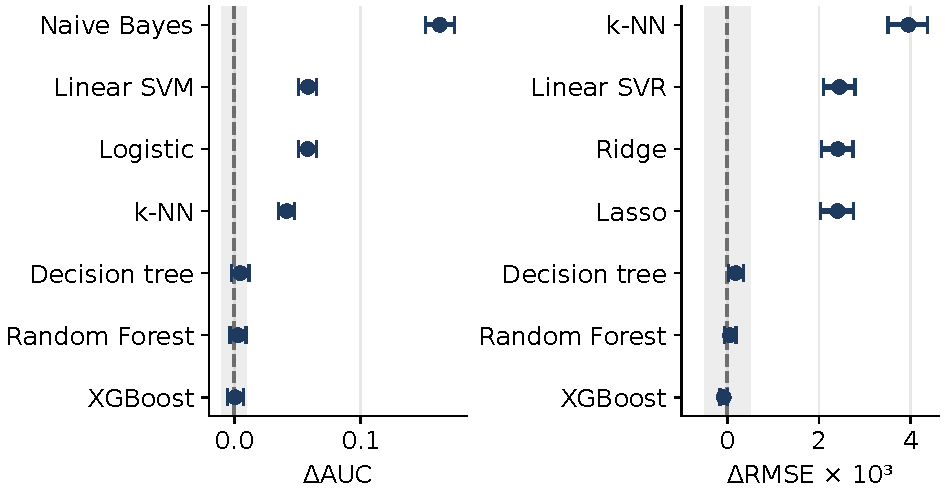
\includegraphics[width=\linewidth]{fig_intervals.pdf}
  \caption{Diferencia de la métrica principal entre la EBM y cada modelo de referencia en la prueba, con su
  intervalo \emph{bootstrap} BCa al 95~\% (2.000 réplicas): AUC (izquierda; positivo favorece a la EBM) y RMSE
  en milésimas (derecha; positivo favorece a la EBM). La banda gris es la región de equivalencia práctica.}
  \label{fig:intervals}
\end{figure}

\subsection{Resultados del estudio de ablación}
\label{sec:ablacion_res}

La tabla~\ref{tab:ablacion} y la figura~\ref{fig:ablation} comparan, con el mismo protocolo y Holm dentro de
cada tarea, las variantes que cambian el modelo con el modelo completo (ponderación, Grid, $K = 0$); la
fidelidad y la semilla no cambian el modelo y se resumen en la tabla~\ref{tab:semillas}.

\begin{enumerate}
  \item \textbf{Sin interacciones.} Como la búsqueda eligió $K = 0$, la variante se evalúa en la EBM de la
        comparación con la entrega anterior (5 pares), que sin pares obtiene 0,7185 de AUC frente a 0,7187
        (DeLong $p = 0{,}91$) y aun así supera a la logística en $+0{,}035$ ($p < 10^{-21}$). Hipótesis
        confirmada: la aditividad basta.
  \item \textbf{Balanceo.} Sin balanceo el AUC de prueba es idéntico (0,8289; probabilidad de equivalencia
        1,0); SMOTE y ADASYN lo bajan en 0,003
        sin significancia ($p$ ajustado 0,55 y 0,70) y multiplican el tiempo de la corrida por 4,4
        y 5,4. Lo que mueve el balanceo es el \emph{recall} con umbral
        0,5: 0,707 con ponderación frente a 0,355 sin ella y 0,34--0,35 con sobremuestreo. Hipótesis
        confirmada: el balanceo elige el punto de operación.
  \item \textbf{Fidelidad de la búsqueda.} En las ocho configuraciones aleatorias, la correlación de Spearman
        entre el AUC con $B = 2$ y con $B = 8$ es 0,83, la ganadora es la misma y la fidelidad
        baja ahorra el 66~\% del tiempo de búsqueda. Hipótesis confirmada.
  \item \textbf{Optimizador.} TPE y la genética llegan, con configuraciones distintas, al mismo AUC que Grid
        ($+0{,}0003$); Random Search queda $0{,}0049$ por debajo en la prueba, sin sobrevivir a Holm
        ($p = 0{,}13$) ni aparecer en los pliegues ($p = 0{,}78$). En regresión los cuatro son equivalentes. En
        las 140 corridas de la guía (tabla~\ref{tab:optimizadores_res}), Friedman rechaza por la métrica final en
        clasificación ($p = 0{,}001$, por Random Search) y no en regresión ($p = 0{,}82$); por el área de
        arrepentimiento la bayesiana tiene el menor rango en las dos tareas (Friedman $p < 10^{-6}$). Hipótesis
        confirmada en su segunda parte (la eficiencia por evaluación distingue a los métodos) y solo en parte en
        la primera: la métrica final no distingue a TPE, Grid y la genética, pero sí a Random Search en
        clasificación.
  \item \textbf{Semilla.} Con cinco semillas, la desviación del AUC de prueba de la EBM es 0,00004 y la del
        RMSE 0,000003 (tabla~\ref{tab:semillas}), de 10 a 100 veces menores que sus diferencias con los modelos
        de árboles. Hipótesis refutada para la EBM, más estable que Random Forest (0,0010) y XGBoost (0,0003),
        para los que sí se sostiene.
\end{enumerate}

\begin{table}[tbp]
  \centering\scriptsize\setlength{\tabcolsep}{1.5pt}
  \caption{Ablación: cada variante cambia un componente de la EBM completa y conserva el resto. Métrica externa (AUC o RMSE; media $\pm$ desviación de los 5 pliegues) y de prueba, \emph{recall} de prueba con umbral 0,5 (clasificación); $\Delta$ entre la variante y el modelo completo en la prueba, orientada para que un valor positivo indique que la variante pierde (AUC$_{\mathrm{comp}} -$ AUC$_{\mathrm{var}}$; en regresión RMSE$_{\mathrm{var}} - $RMSE$_{\mathrm{comp}}$ en milésimas), con intervalo BCa; $p$ de la $t$ corregida sobre los pliegues y de DeLong o Diebold-Mariano sobre la prueba, ajustados por Holm dentro de cada tarea ($^{*}$: comparación única, sin ajustar); probabilidad bayesiana de equivalencia (ROPE) entre la variante y el modelo completo. La variante sin interacciones se evalúa en la partición y la etiqueta de la comparación con la entrega anterior, donde la búsqueda sí eligió pares.}
  \label{tab:ablacion}
  \begin{tabular}{@{}>{\raggedright\arraybackslash}p{0.26\linewidth} c c c c c c c@{}}
    \toprule
    Variante & Métrica externa & Prueba & Recall$_{0{,}5}$ & $\Delta$ [IC 95~\%] & $p$ $t$ corr. & $p$ prueba & $P$(ROPE) \\
    \midrule
    EBM completa (ponderación, Grid, $K=0$) & $0{,}8292$ $\pm$ $0{,}0037$ & $0{,}8289$ & $0{,}707$ & -- & -- & -- & -- \\
    balanceo: sin balanceo (Grid) & $0{,}8285$ $\pm$ $0{,}0035$ & $0{,}8289$ & $0{,}355$ & $0{,}0000$ [$-0{,}0006$; $0{,}0006$] & $0{,}511$ & $1{,}000$ & $1{,}000$ \\
    balanceo: SMOTE (Grid) & $0{,}8278$ $\pm$ $0{,}0032$ & $0{,}8258$ & $0{,}346$ & $+0{,}0031$ [$-0{,}0008$; $0{,}0069$] & $0{,}511$ & $0{,}549$ & $1{,}000$ \\
    balanceo: ADASYN (Grid) & $0{,}8280$ $\pm$ $0{,}0033$ & $0{,}8263$ & $0{,}336$ & $+0{,}0026$ [$-0{,}0012$; $0{,}0064$] & $0{,}496$ & $0{,}702$ & $1{,}000$ \\
    optimizador: Random (ponderación) & $0{,}8276$ $\pm$ $0{,}0024$ & $0{,}8240$ & $0{,}950$ & $+0{,}0049$ [$0{,}0007$; $0{,}0092$] & $0{,}783$ & $0{,}125$ & $0{,}998$ \\
    optimizador: TPE (ponderación) & $0{,}8287$ $\pm$ $0{,}0041$ & $0{,}8286$ & $0{,}715$ & $+0{,}0003$ [$-0{,}0004$; $0{,}0010$] & $0{,}783$ & $1{,}000$ & $1{,}000$ \\
    optimizador: Genética (ponderación) & $0{,}8281$ $\pm$ $0{,}0036$ & $0{,}8287$ & $0{,}712$ & $+0{,}0003$ [$-0{,}0004$; $0{,}0009$] & $0{,}783$ & $1{,}000$ & $1{,}000$ \\
    sin interacciones ($K=0$) frente a la EBM con 5 pares (TPE) & -- & $0{,}7185$ & -- & $+0{,}0002$ [$-0{,}0029$; $0{,}0030$] & -- & $0{,}910$$^{*}$ & -- \\
    \midrule
    EBM completa (Grid, $K=0$) & $0{,}0590$ $\pm$ $0{,}0004$ & $0{,}0593$ & -- & -- & -- & -- & -- \\
    optimizador: Random & $0{,}0591$ $\pm$ $0{,}0004$ & $0{,}0592$ & -- & $-0{,}01$ [$-0{,}05$; $0{,}04$] & $0{,}581$ & $1{,}000$ & $1{,}000$ \\
    optimizador: TPE & $0{,}0590$ $\pm$ $0{,}0004$ & $0{,}0593$ & -- & $+0{,}03$ [$-0{,}02$; $0{,}09$] & $0{,}581$ & $0{,}884$ & $1{,}000$ \\
    optimizador: Genética & $0{,}0591$ $\pm$ $0{,}0004$ & $0{,}0593$ & -- & $+0{,}01$ [$-0{,}03$; $0{,}06$] & $0{,}581$ & $1{,}000$ & $1{,}000$ \\
    \bottomrule
  \end{tabular}
\end{table}

\begin{table}[tbp]
  \centering\scriptsize\setlength{\tabcolsep}{3pt}
  \caption{Sensibilidad a la semilla: modelos finales reentrenados con distintas semillas (los datos no cambian) y búsqueda del árbol de decisión repetida con cinco semillas de cada optimizador estocástico; media y desviación de la métrica de prueba.}
  \label{tab:semillas}
  \begin{tabular}{@{}l l r l c c@{}}
    \toprule
    Tarea & Modelo & Semillas & Métrica & Media & Desviación \\
    \midrule
    Clasificación & EBM (propuesto) & 5 & AUC & $0{,}8288$ & $0{,}00004$ \\
    Clasificación & Random Forest & 5 & AUC & $0{,}8281$ & $0{,}00101$ \\
    Clasificación & SVM lineal & 10 & AUC & $0{,}7706$ & $0{,}00000$ \\
    Clasificación & XGBoost & 10 & AUC & $0{,}8282$ & $0{,}00029$ \\
    Regresión & EBM (propuesto) & 5 & RMSE & $0{,}0593$ & $0{,}000003$ \\
    Regresión & Random Forest & 5 & RMSE & $0{,}0593$ & $0{,}000009$ \\
    Regresión & XGBoost & 10 & RMSE & $0{,}0592$ & $0{,}000006$ \\
    Clasificación & Árbol, búsqueda con TPE & 5 & AUC & $0{,}8246$ & $0{,}00221$ \\
    Clasificación & Árbol, búsqueda con Genética & 5 & AUC & $0{,}8243$ & $0{,}00087$ \\
    Clasificación & Árbol, búsqueda con Random & 5 & AUC & $0{,}8252$ & $0{,}00254$ \\
    \bottomrule
  \end{tabular}
  \par\smallskip\begin{minipage}{0.97\linewidth}\scriptsize Multi-fidelidad de la EBM: 8 configuraciones aleatorias evaluadas con $B=2$ y $B=8$; $\rho$ de Spearman entre los dos AUC $0{,}833$, misma configuración ganadora (sí), ahorro de tiempo de búsqueda $66$~\%.\end{minipage}
\end{table}

\begin{table}[tbp]
  \centering\small\setlength{\tabcolsep}{3pt}
  \caption{Los cuatro optimizadores con el mismo presupuesto, en los bloques modelo $\times$ balanceo con las cuatro búsquedas completas de las 140 corridas de la guía (27 en clasificación, 7 en regresión; las de la EBM se excluyen): rango medio por la métrica externa (1 = mejor), bloques ganados, segundos por evaluación, área media bajo la curva de arrepentimiento normalizado (menor es mejor) y evaluaciones hasta cerrar el 95~\% de la brecha, estas dos últimas tal como las publicó el Entregable 3.}
  \label{tab:optimizadores_res}
  \begin{tabular}{@{}l l r r r r r@{}}
    \toprule
    Tarea & Método & Rango & Victorias & s/eval. & Área arrep. & Evals.\ 95~\% \\
    \midrule
    Clas. & Grid & $2{,}22$ & 12 & $2{,}61$ & $0{,}234$ & $14{,}2$ \\
    Clas. & Random & $3{,}22$ & 4 & $2{,}46$ & $0{,}171$ & $7{,}2$ \\
    Clas. & TPE & $2{,}63$ & 2 & $4{,}48$ & $0{,}123$ & $10{,}3$ \\
    Clas. & Genética & $1{,}93$ & 15 & $4{,}27$ & $0{,}137$ & $13{,}1$ \\
    \midrule
    Regr. & Grid & $2{,}71$ & 2 & $2{,}43$ & $0{,}181$ & $9{,}9$ \\
    Regr. & Random & $2{,}71$ & 0 & $2{,}05$ & $0{,}041$ & $7{,}4$ \\
    Regr. & TPE & $2{,}14$ & 2 & $2{,}94$ & $0{,}038$ & $5{,}5$ \\
    Regr. & Genética & $2{,}43$ & 3 & $3{,}37$ & $0{,}057$ & $7{,}4$ \\
    \bottomrule
  \end{tabular}
\end{table}


\begin{figure}[tbp]
  \centering
  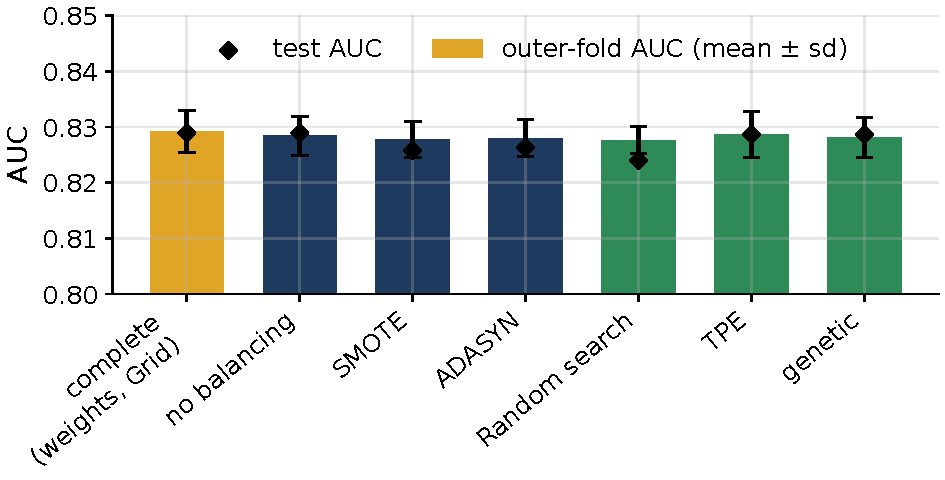
\includegraphics[width=\linewidth]{fig_ablation.pdf}
  \caption{Ablación en clasificación: AUC externa (media $\pm$ desviación de los 5 pliegues; barras) y AUC de
  prueba (rombos) del modelo completo y de cada variante de balanceo (azul) y de optimizador (verde).}
  \label{fig:ablation}
\end{figure}

\subsection{Sensibilidad y robustez}
\label{sec:sensibilidad}

La tabla~\ref{tab:semillas} y las figuras~\ref{fig:sensitivity} y~\ref{fig:hyper} reúnen las fuentes de
variabilidad. La semilla del modelo apenas pesa; la del optimizador pesa más: repetir la
búsqueda del árbol con cinco semillas mueve el AUC de prueba en 0,0009 a 0,0025, el orden de las diferencias
entre optimizadores. La sensibilidad a los hiperparámetros es baja: variando uno a la vez desde la configuración final, con validación cruzada de 3 pliegues y $B = 2$, el
AUC se mueve entre 0,8267 y 0,8292 (figura~\ref{fig:hyper}); el más influyente es el número de interacciones.
Las 16 corridas de clasificación de la EBM terminan con configuraciones muy distintas
(figura~\ref{fig:sensitivity}) y un AUC externo entre 0,8276 y 0,8292, un rango menor que la desviación entre
pliegues. La curva de aprendizaje,
ajustada con el modelo final sobre subconjuntos del entrenamiento y evaluada en la prueba, sube de 0,8234 con
2.500 clientes a 0,8288 con 38.978, y desde 10.000 solo gana 0,0018: con 2.500 clientes la EBM ya supera a la
logística entrenada con todos (0,771), mientras que el árbol es el más dependiente del tamaño; las curvas de
referencia provienen del experimento de escalamiento del Entregable 3, fuera del
pipeline anidado, por lo que Random Forest termina 0,003 por encima de su modelo final. La robustez al
desbalance se midió con y sin remuestreo (ablación): el AUC no cambia. La validación anidada predice la
prueba casi sin sesgo: en las 124 corridas de clasificación la correlación entre el AUC externo y el de
prueba es 0,997 y la diferencia media $+0{,}0016$.

\begin{figure}[tbp]
  \centering
  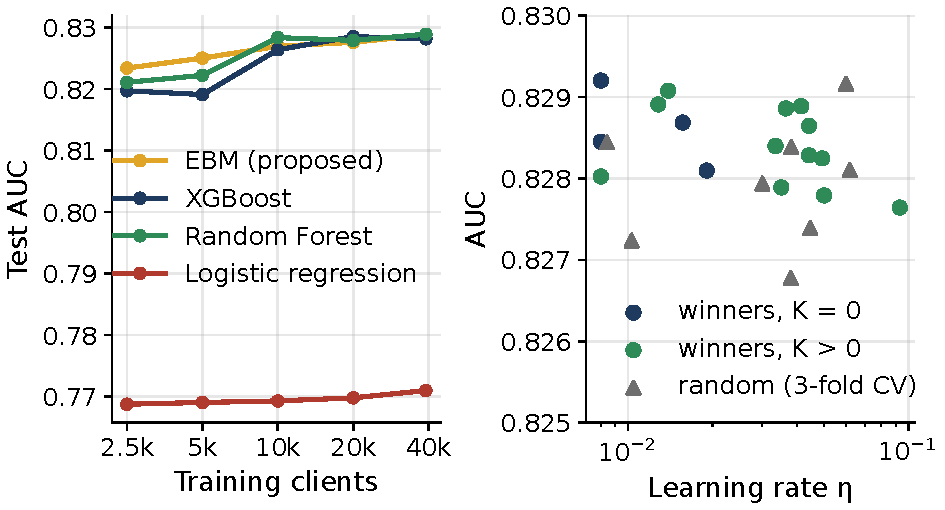
\includegraphics[width=\linewidth]{fig_sensitivity.pdf}
  \caption{Izquierda: curva de aprendizaje (AUC de prueba frente al número de clientes de entrenamiento, con
  los hiperparámetros finales de cada modelo; la EBM se ajusta en el guion de esta sección y las referencias
  provienen del experimento de escalamiento del Entregable 3). Derecha: AUC de la EBM frente a la tasa de
  aprendizaje en las 16 configuraciones ganadoras de las corridas (círculos; azul $K = 0$, verde $K > 0$; AUC
  externo) y en las ocho configuraciones aleatorias de la prueba de fidelidad (triángulos; validación cruzada de
  3 pliegues con $B = 8$).}
  \label{fig:sensitivity}
\end{figure}

\begin{figure}[tbp]
  \centering
  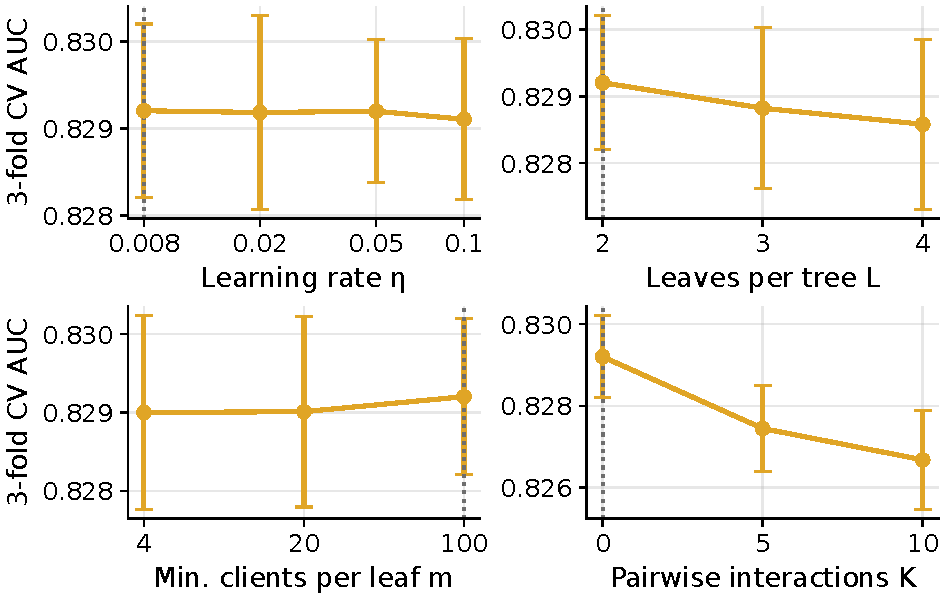
\includegraphics[width=\linewidth]{fig_hyper.pdf}
  \caption{Sensibilidad de la EBM a cada hiperparámetro por separado: AUC (media $\pm$ desviación de una
  validación cruzada de 3 pliegues sobre el entrenamiento, con $B = 2$) al variar la tasa de aprendizaje, las
  hojas por árbol, el mínimo de clientes por hoja y el número de interacciones desde la configuración final
  (línea punteada).}
  \label{fig:hyper}
\end{figure}

\subsection{Costo computacional}
\label{sec:costo}

Según la tabla~\ref{tab:costo}, la EBM es el modelo más lento de ajustar: 26,7~s en clasificación y 31,8~s en
regresión, 17 y 15 veces más que XGBoost (1,6 y 2,1~s) y del orden de Random Forest. En inferencia está en el
grupo rápido (0,067~s para los 9.745 clientes, tres veces menos que Random Forest y cien menos que k-NN),
ocupa 1,5~MB frente a 44~MB del bosque, guarda 15.485 valores frente a 574.556 nodos y
necesita 20~MB de memoria pico en el ajuste frente a 68~MB del bosque. La EBM no mejora el AUC de XGBoost y
cuesta 17 veces más en ajuste, pero el ajuste ocurre una vez y la consulta es igual de barata; el costo extra
compra un modelo legible sin explicador.

\begin{table}[tbp]
  \centering\scriptsize\setlength{\tabcolsep}{3pt}
  \caption{Costo computacional de la mejor combinación de cada modelo en el equipo de referencia (AMD de 6 núcleos, 15,9~GB): ajuste del modelo final sobre los 38.978 clientes y puntuación de los 9.745 de prueba (mediana de 3 y 5 repeticiones con el pipeline completo), duración de la corrida anidada completa, tamaño serializado, número de parámetros (valores almacenados: nodos de los árboles, puntajes de las funciones de forma, coeficientes; k-NN guarda la matriz de entrenamiento) y memoria pico del ajuste por encima de la base: en clasificación la midió el Entregable 3 (la de la EBM se midió aquí, mediana de tres ajustes) y en regresión se midió aquí para todos.}
  \label{tab:costo}
  \begin{tabular}{@{}l l r r r r r r@{}}
    \toprule
    Tarea & Modelo & Ajuste (s) & Inferencia (s) & Corrida (min) & Tamaño (MB) & Parámetros & Memoria (MB) \\
    \midrule
    Clas. & k-NN & $0{,}28$ & $7{,}164$ & $34{,}7$ & $23{,}50$ & 3.040.284 & $<1$ \\
    Clas. & Naive Bayes & $0{,}30$ & $0{,}068$ & $0{,}7$ & $0{,}01$ & 314 & $24$ \\
    Clas. & SVM lineal & $0{,}92$ & $0{,}052$ & $2{,}1$ & $<0{,}01$ & 79 & $32$ \\
    Clas. & Árbol de decisión & $1{,}38$ & $0{,}054$ & $1{,}8$ & $0{,}01$ & 53 & $12$ \\
    Clas. & XGBoost & $1{,}61$ & $0{,}060$ & $8{,}9$ & $0{,}56$ & 14.063 & $13$ \\
    Clas. & Regresión logística & $1{,}83$ & $0{,}056$ & $3{,}1$ & $<0{,}01$ & 79 & $61$ \\
    Clas. & Random Forest & $23{,}65$ & $0{,}187$ & $20{,}9$ & $43{,}97$ & 574.556 & $68$ \\
    Clas. & \textbf{EBM (propuesto)} & $26{,}72$ & $0{,}067$ & $18{,}7$ & $1{,}49$ & 15.485 & $20$ \\
    \midrule
    Regr. & k-NN & $0{,}25$ & $4{,}725$ & $24{,}9$ & $23{,}50$ & 3.040.284 & $<1$ \\
    Regr. & Ridge & $0{,}28$ & $0{,}046$ & $1{,}5$ & $<0{,}01$ & 79 & $24$ \\
    Regr. & Lasso & $0{,}46$ & $0{,}046$ & $6{,}7$ & $<0{,}01$ & 79 & $23$ \\
    Regr. & SVR lineal & $0{,}66$ & $0{,}046$ & $2{,}7$ & $<0{,}01$ & 79 & $29$ \\
    Regr. & Árbol de decisión & $0{,}84$ & $0{,}047$ & $3{,}7$ & $0{,}01$ & 71 & $12$ \\
    Regr. & XGBoost & $2{,}09$ & $0{,}065$ & $10{,}4$ & $0{,}46$ & 3.582 & $5$ \\
    Regr. & Random Forest & $12{,}31$ & $0{,}145$ & $16{,}1$ & $6{,}01$ & 85.948 & $13$ \\
    Regr. & \textbf{EBM (propuesto)} & $31{,}85$ & $0{,}054$ & $26{,}6$ & $1{,}49$ & 15.485 & $25$ \\
    \bottomrule
  \end{tabular}
\end{table}


\subsection{Interpretabilidad y análisis de errores}
\label{sec:errores}

\paragraph{Qué usa el modelo.}
La tabla~\ref{tab:importancia} ordena los términos de la EBM de clasificación: la edad (37,8~\%), la
frecuencia de uso de la aplicación (30,1~\%), la satisfacción (11,6~\%) y la satisfacción de base (2,5~\%)
reúnen el 82~\% de la importancia, y la importancia por permutación en la prueba coincide (caídas de AUC de
0,177 a 0,0008; ningún otro predictor llega a 0,0003). Son las cuatro variables del
análisis exploratorio y las que SHAP \citep{lundberg2017shap} señala en XGBoost en el Entregable 3. Las
funciones de forma (figura~\ref{fig:shapes}) muestran la no linealidad que los modelos lineales no captan: la
edad no es monótona (de $-1{,}57$ a $+1{,}40$ en el logit), la frecuencia de uso reduce el riesgo con fuerza
hasta unos 20 inicios de sesión y luego se aplana, la satisfacción actúa por escalones y la de base sigue una
curva en S.

\paragraph{Dónde falla.}
La tabla~\ref{tab:errores} divide la prueba por cohorte de edad y por \ap, la variable excluida. La cohorte de
59--60 años, con el 46~\% de riesgo alto, es la más difícil (AUC 0,645 dentro de la cohorte); la de 44--45
(9~\%) la más fácil (0,922). La EBM y XGBoost alcanzan el mismo \emph{recall} global con clientes distintos:
con la capacidad del 25~\%, la EBM contacta sobre todo a la cohorte mayor (deja fuera al 37~\% de sus
clientes de riesgo alto, pero al 91~\% de los de 44--45) y XGBoost reparte más (56~\% y 34~\%), porque la edad domina al modelo aditivo; de los
1.171 clientes de riesgo alto que la EBM deja fuera, 563 son de 59--60 años, 354 de 29--30 y 254 de 44--45.
Por \ap, en cambio, el AUC dentro de cada nivel está entre 0,988 y 0,999 en los dos modelos y el sesgo de la
regresión forma una escalera: $-0{,}055$ con un producto, $-0{,}005$ con dos, $+0{,}045$, $+0{,}095$ y
$+0{,}145$ con tres, cuatro y cinco. El modelo pronostica a todos cerca del nivel de dos productos porque no
ve cuántos tienen; los errores grandes son la parte del objetivo que depende de la variable excluida y explican
la compresión y la asimetría de la figura~\ref{fig:regression}. La tabla~\ref{tab:ejemplos} muestra tres
clientes representativos de esos errores; en los dos primeros la edad y el uso de la aplicación apuntan en
sentido contrario al nivel de \ap, que decide el puntaje real.

\begin{table}[tbp]
  \centering\small\setlength{\tabcolsep}{3pt}
  \caption{Interpretabilidad de la EBM de clasificación: cuota de la importancia de cada término (media del valor absoluto de su función de forma sobre el entrenamiento; los 78 términos suman 100~\%) e importancia por permutación sobre la prueba (caída media $\pm$ desviación del AUC al permutar cada predictor original, 5 repeticiones).}
  \label{tab:importancia}
  \begin{tabular}{@{}l r l c@{}}
    \toprule
    Término (EBM) & Cuota & Predictor permutado & Caída del AUC \\
    \midrule
    \texttt{age} & $37{,}8$~\% & \texttt{age} & $0{,}1772$ $\pm$ $0{,}0050$ \\
    \texttt{app\_logins\_frequency} & $30{,}1$~\% & \texttt{app\_logins\_frequency} & $0{,}1159$ $\pm$ $0{,}0062$ \\
    \texttt{satisfaction\_score} & $11{,}6$~\% & \texttt{satisfaction\_score} & $0{,}0282$ $\pm$ $0{,}0021$ \\
    \texttt{base\_satisfaction} & $2{,}5$~\% & \texttt{base\_satisfaction} & $0{,}0008$ $\pm$ $0{,}0005$ \\
    \texttt{income\_bracket\_Low} & $1{,}5$~\% & \texttt{prop\_Transfer} & $0{,}0002$ $\pm$ $0{,}0001$ \\
    \texttt{prop\_Withdrawal} & $1{,}0$~\% & \texttt{customer\_tenure} & $0{,}0002$ $\pm$ $0{,}0001$ \\
    \texttt{product\_satisfaction} & $0{,}9$~\% & \texttt{credit\_utilization\_ratio} & $0{,}0001$ $\pm$ $0{,}0001$ \\
    \texttt{investment\_account} & $0{,}8$~\% & \texttt{investment\_account} & $0{,}0001$ $\pm$ $0{,}0000$ \\
    \bottomrule
  \end{tabular}
\end{table}

\begin{table}[tbp]
  \centering\scriptsize\setlength{\tabcolsep}{2pt}
  \caption{Análisis de errores en la prueba por cohorte de edad y por número de productos activos (variable excluida del modelo): tamaño, prevalencia de riesgo alto, AUC de la EBM y de XGBoost dentro del segmento, fracción de clientes de riesgo alto que cada modelo deja fuera del 25~\% contactado (FN, falsos negativos), RMSE de regresión de los dos modelos y sesgo medio del pronóstico de la EBM (pronóstico $-$ real).}
  \label{tab:errores}
  \begin{tabular}{@{}l r r c c c c c c c@{}}
    \toprule
    Segmento & $n$ & Prev. & AUC EBM & AUC XGB & FN EBM & FN XGB & RMSE EBM & RMSE XGB & Sesgo EBM \\
    \midrule
    cohorte de edad 29--30 & 3.224 & $18$~\% & $0{,}830$ & $0{,}840$ & $60$~\% & $38$~\% & $0{,}0598$ & $0{,}0598$ & $+0{,}001$ \\
    cohorte de edad 44--45 & 3.174 & $9$~\% & $0{,}922$ & $0{,}930$ & $91$~\% & $34$~\% & $0{,}0586$ & $0{,}0584$ & $0{,}000$ \\
    cohorte de edad 59--60 & 3.347 & $46$~\% & $0{,}645$ & $0{,}636$ & $37$~\% & $56$~\% & $0{,}0594$ & $0{,}0593$ & $0{,}000$ \\
    \midrule
    productos activos 1 & 3.918 & $54$~\% & $0{,}997$ & $0{,}999$ & $55$~\% & $55$~\% & $0{,}0548$ & $0{,}0548$ & $-0{,}055$ \\
    productos activos 2 & 2.939 & $9$~\% & $0{,}996$ & $0{,}995$ & $0$~\% & $0$~\% & $0{,}0067$ & $0{,}0057$ & $-0{,}005$ \\
    productos activos 3 & 1.390 & $0$~\% & $0{,}999$ & $0{,}988$ & $0$~\% & $0$~\% & $0{,}0456$ & $0{,}0453$ & $+0{,}045$ \\
    productos activos 4 & 1.016 & $0$~\% & -- & -- & -- & -- & $0{,}0954$ & $0{,}0953$ & $+0{,}095$ \\
    productos activos 5 & 482 & $0$~\% & -- & -- & -- & -- & $0{,}1453$ & $0{,}1453$ & $+0{,}145$ \\
    \bottomrule
  \end{tabular}
\end{table}

\begin{table}[tbp]
  \centering\scriptsize\setlength{\tabcolsep}{3pt}
  \caption{Tres clientes de prueba representativos de los errores: el de riesgo alto con menor puntaje de la EBM (FN, el falso negativo más grave), el de riesgo bajo con mayor puntaje (FP, el falso positivo más grave) y el de mayor error absoluto de regresión, con sus variables de señal, el nivel de \ap\ (que el modelo no ve), su puntaje real y las predicciones de la EBM y de XGBoost.}
  \label{tab:ejemplos}
  \begin{tabular}{@{}l c c c@{}}
    \toprule
    Variable & FN más grave & FP más grave & Mayor error de regresión \\
    \midrule
    Edad (años) & 44 & 60 & 44 \\
    Inicios de sesión & $22$ & $4$ & $37$ \\
    Satisfacción & $3$ & $3$ & $4$ \\
    \ap & 1 & 4 & 5 \\
    Riesgo alto real & sí & no & no \\
    Puntaje real & $0{,}393$ & $0{,}351$ & $0{,}153$ \\
    Prob. EBM / XGBoost & $0{,}206$ / $0{,}590$ & $0{,}988$ / $0{,}648$ & $0{,}075$ / $0{,}315$ \\
    Pron. EBM / XGBoost & $0{,}334$ / $0{,}341$ & $0{,}442$ / $0{,}440$ & $0{,}311$ / $0{,}305$ \\
    \bottomrule
  \end{tabular}
\end{table}


\begin{figure}[tbp]
  \centering
  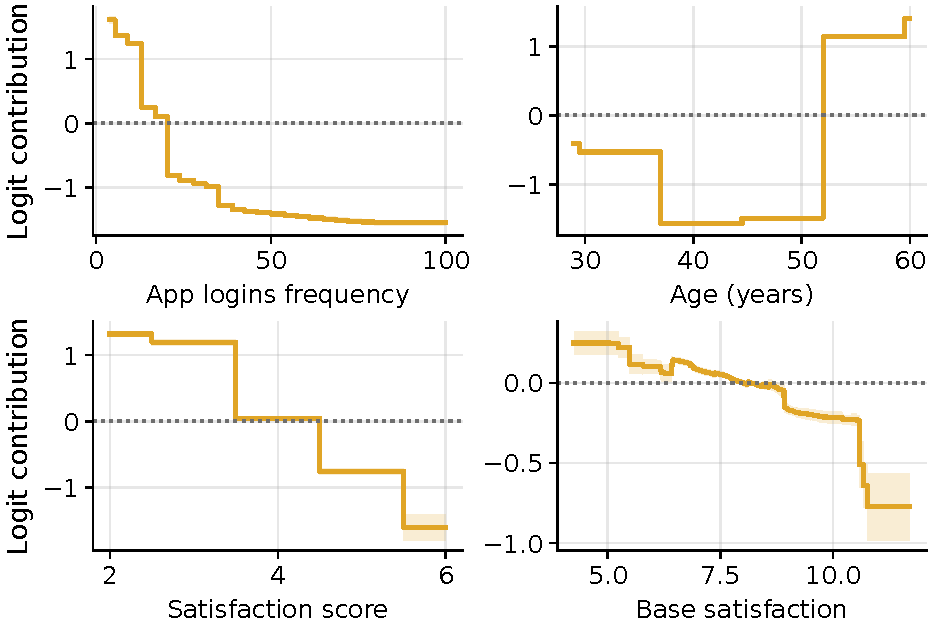
\includegraphics[width=\linewidth]{fig_shapes.pdf}
  \caption{Funciones de forma de la EBM de clasificación para las cuatro variables con señal: contribución al
  logit del riesgo alto (centrada) con la banda entre las 8 bolsas externas, en las unidades originales de cada
  variable.}
  \label{fig:shapes}
\end{figure}

\subsection{Discusión, limitaciones y amenazas a la validez}
\label{sec:discusion}

Los resultados sugieren que, en este problema, un modelo aditivo con funciones de forma alcanza la misma
capacidad predictiva que los ensambles de árboles: la EBM empata con XGBoost, Random Forest y el árbol en las
dos tareas y supera con claridad a los modelos lineales, a k-NN y a Naive Bayes, como en \citet{lou2013ga2m}.
La ablación explica por qué aquí ni siquiera hacen
falta las interacciones: la señal está en cuatro variables con efectos no lineales y casi independientes, de
modo que lo que faltaba en la entrega anterior era flexibilidad por variable, no profundidad. El empate con
XGBoost es una propiedad de los datos: el techo de información sin \ap\ estimado en el Entregable 3 es 0,7223
de AUC (etiqueta de la mediana) y 0,2197 de $R^2$, y la EBM cubre el 98~\% de ambos ($\auc - 0{,}5$).

Hay un solo conjunto de datos, con rasgos sintéticos (cohortes de edad, escalera de productos activos), y el
objetivo es el puntaje de otro modelo, no la fuga observada. Con cinco pliegues la $t$ corregida tiene 4 grados de libertad y poca potencia, y McNemar en el punto
de operación es insensible a diferencias que el AUC sí ve. Otras amenazas son menores: el SVM es lineal (el núcleo RBF multiplicaba por
70 el costo), la logística cubre L1 y L2 como un solo modelo, la regresión no incluye un modelo bayesiano, los
tiempos son de un solo equipo y, aunque las variables derivadas no usan el objetivo, en un conjunto sintético
no puede descartarse una fuga residual. La conclusión proporcional a la evidencia es que la EBM es una
alternativa equivalente a XGBoost en precisión, más lenta de ajustar, igual de rápida en inferencia y legible
por construcción; no que sea mejor.

% Conclusiones del informe final. Las cifras provienen de la sección de resultados.
\section{Conclusiones}
\label{sec:conclusiones}

El proyecto partió de una pregunta: si un modelo aditivo legible alcanza en COFINFAD la precisión de los
ensambles de árboles, y a qué costo. La respuesta de la sección~\ref{sec:resultados} es que la alcanza, no la
supera. La EBM obtiene el mayor AUC de prueba de los ocho modelos de clasificación (0,8289) y el segundo RMSE de
regresión (0,05925, a 0,00008 de XGBoost); supera con significación estadística, en todas las pruebas y tras la
corrección de Holm, a los modelos lineales, a k-NN y a Naive Bayes (cuatro de las siete referencias de cada
tarea); y frente a XGBoost, Random Forest y el árbol de decisión ninguna prueba al 5~\% encuentra diferencia:
la probabilidad de equivalencia práctica va de 0,94 a 0,997 en clasificación y es 0,9998 con XGBoost en
regresión, y solo el \emph{Model Confidence Set} al 90~\% detecta una ventaja sistemática de XGBoost de
décimas de milésima de RMSE. Frente a la entrega anterior, en su misma partición y etiqueta, la EBM sube el AUC
de 0,6832 a 0,7187 y baja el RMSE de 0,06166 a 0,05926 ($p < 0{,}001$), y cubre el 98~\% del techo de
información que deja la exclusión de \ap: el empate entre los modelos flexibles es una propiedad de los datos,
no una debilidad del modelo.

El estudio de ablación cerró sus cinco hipótesis. Se confirmó que la aditividad basta (sin interacciones se
pierden 0,0002 de AUC, $p = 0{,}91$), que el balanceo no cambia el AUC y solo desplaza el punto de operación (el
\emph{recall} con umbral 0,5 pasa de 0,355 a 0,707 con ponderación, al mismo AUC), que la búsqueda de baja
fidelidad conserva el orden de las configuraciones y ahorra el 66~\% del tiempo, y que la eficiencia por
evaluación sí distingue a los optimizadores (la bayesiana tiene el menor arrepentimiento) aunque la métrica
final solo separe a Random Search en clasificación. Se refutó, en cambio, la hipótesis de que la variabilidad
por semilla fuera del orden de las diferencias entre modelos: la EBM es casi determinista (desviación de
0,00004 de AUC), más estable que Random Forest y XGBoost. La sensibilidad a los hiperparámetros es baja (AUC
entre 0,8267 y 0,8292 al variarlos uno a uno) y la validación anidada predijo la prueba casi sin sesgo
(correlación 0,997 en 124 corridas), de modo que las conclusiones no dependen de una configuración afortunada.

Dos lecciones son prácticas. La primera es que la significancia estadística no es relevancia práctica: con la
capacidad de campaña del 25~\% todos los modelos salvo Naive Bayes identifican casi a los mismos clientes (la
EBM 1.228 de los 2.399 de riesgo alto y la regresión logística 1.225), aunque el AUC los separe con
$p < 0{,}001$; la ventaja de los modelos flexibles aparece en otras capacidades (con el 50~\% capturan el 91~\%
de la fuga frente al 77~\% de la logística), así que el modelo debe elegirse con la capacidad de la campaña en
mente y con las probabilidades recalibradas (el ECE baja de 0,170 a 0,003--0,010 con regresión isotónica). La
segunda es el costo: la EBM es el modelo más lento de ajustar (26,7~s, de 15 a 17 veces XGBoost), pero su
inferencia sobre los 9.745 clientes de prueba tarda 0,067~s, como XGBoost, y ocupa 1,5~MB; para una campaña
que ajusta el modelo una vez y lo consulta sobre toda la cartera, el costo relevante es el de inferencia. Lo que
el ajuste más caro compra es la legibilidad: cuatro variables reúnen el 82~\% de la importancia y sus funciones
de forma muestran directamente la no linealidad que los modelos lineales no captan (la edad no monótona, la
meseta de la frecuencia de uso, los escalones de la satisfacción), sin explicador auxiliar. El análisis de
errores localizó los fallos: la cohorte de 59--60 años, con el 46~\% de riesgo alto, es la más difícil, y los
errores grandes de la regresión siguen una escalera por número de productos activos, es decir, son la parte del
objetivo que depende de la variable excluida y que ningún modelo puede recuperar sin ella.

Las limitaciones acotan estas conclusiones. Hay un único conjunto de datos, con rasgos sintéticos (tres
cohortes de edad, una escalera de productos activos, transacciones sin señal), y el objetivo es el puntaje de
otro modelo, no la fuga observada, de modo que lo aprendido es a reproducir ese puntaje. Con cinco pliegues la
$t$ corregida tiene cuatro grados de libertad y poca potencia, McNemar en el punto de operación es insensible a
las diferencias que el AUC sí ve, el SVM es lineal, la regresión no incluye un modelo bayesiano, los tiempos son
de un solo equipo, y la $t$ corregida, McNemar, el análisis bayesiano y los estudios de sensibilidad se
añadieron después de ver la prueba y se declaran exploratorios. Como trabajo futuro se propone validar en el
tiempo con datos reales de fuga observada (entrenar con un periodo y probar con el siguiente), incorporar el
costo de cada acción de retención para fijar el umbral y la capacidad, acelerar el ajuste de la EBM con una
parada temprana más exigente o restringiendo los predictores a los que tienen señal, aumentar la potencia de las
pruebas pareadas con validación cruzada repetida, y explotar las secuencias de transacciones con modelos que las
traten como series.


\bibliographystyle{elsarticle-harv}
\bibliography{referencias}

\end{document}
